\chapter*{Annexe : Implémentation du Module de Chat}
\addcontentsline{toc}{chapter}{Implémentation du Module de Chat}
\markboth{Implémentation du Module de Chat}{Implémentation du Module de Chat}

%changer le format des sections, sections pour apparaittre sans le num de chapitre
\makeatletter
\renewcommand{\thesection}{\@arabic\c@section}
\makeatother

%recommencer la numérotation des section à "1"
\setcounter{section}{0}

Cette annexe présente les détails sur l'implémentation d'une fonctionnalité en particulier : le système de chat.

\vspace{0.35cm}

Pour constituer le module de chat nous avons utilisé les technologies Socket.io , peerjs.

Dans ce projet, l'implémentation combine deux paradigmes de communication : \verb|REST API| et \verb|WebSocket| avec Socket.io.

\begin{itemize}
    \item  \verb|REST API (Representational State Transfer)| est un style architectural pour les services web qui repose sur des requêtes HTTP classiques. Ce paradigme suit un modèle \textbf{stateless}, où chaque requête est indépendante et doit contenir toutes les informations nécessaires pour son traitement. Les \textbf{REST API} sont utilisées pour gérer des échanges de données simples, comme la récupération ou la modification d'informations sur le serveur.
    \item \verb|WebSocket|, quant à lui, est un protocole de communication bidirectionnelle qui permet d'établir une connexion persistante entre le client et le serveur. Contrairement aux requêtes HTTP classiques, \textbf{WebSocket} permet au serveur d'envoyer des données au client de manière instantanée sans que ce dernier n'ait besoin de faire une nouvelle requête. Ce paradigme est idéal pour les applications nécessitant des mises à jour en temps réel, telles que les chats, les notifications ou les jeux multijoueurs. \textbf{Socket.io} est une bibliothèque JavaScript qui facilite l'implémentation de \textbf{WebSocket} et permet de gérer les événements en temps réel entre le serveur et le client.
\end{itemize}

\vspace{0.35cm}

D'une part, nous utilisons REST API pour gérer les échanges classiques de données entre le client et le serveur, permettant ainsi de manipuler les ressources de manière stateless via des requêtes HTTP standard. Ce modèle est idéal pour les opérations simples telles que la récupération d'informations ou la gestion d'entités.

\vspace{0.35cm}

D'autre part, Socket.io est intégré pour les fonctionnalités nécessitant une communication en temps réel. Grâce à sa capacité à maintenir des connexions persistantes et bidirectionnelles, Socket.io facilite la gestion des événements en temps réel, tels que les notifications, les chats en direct, ou les mises à jour instantanées. Cette approche hybride permet de tirer parti des avantages de chaque technologie selon les besoins spécifiques de l'application.

\clearpage

\section{Module de Chat - Implémentation Côté Backend}

La première étape côté backend a consisté à établir les tables selon le diagramme de classes présenté plus haut à la \autoref{subsection_package_communication}. Cette implémentation repose sur l'architecture présentée à la \autoref{architecture_backend} plus haut.

Les extraits de code ci-dessous permettent l'implémentation des classes essentielles.


\begin{figure}[H]
    \centering
    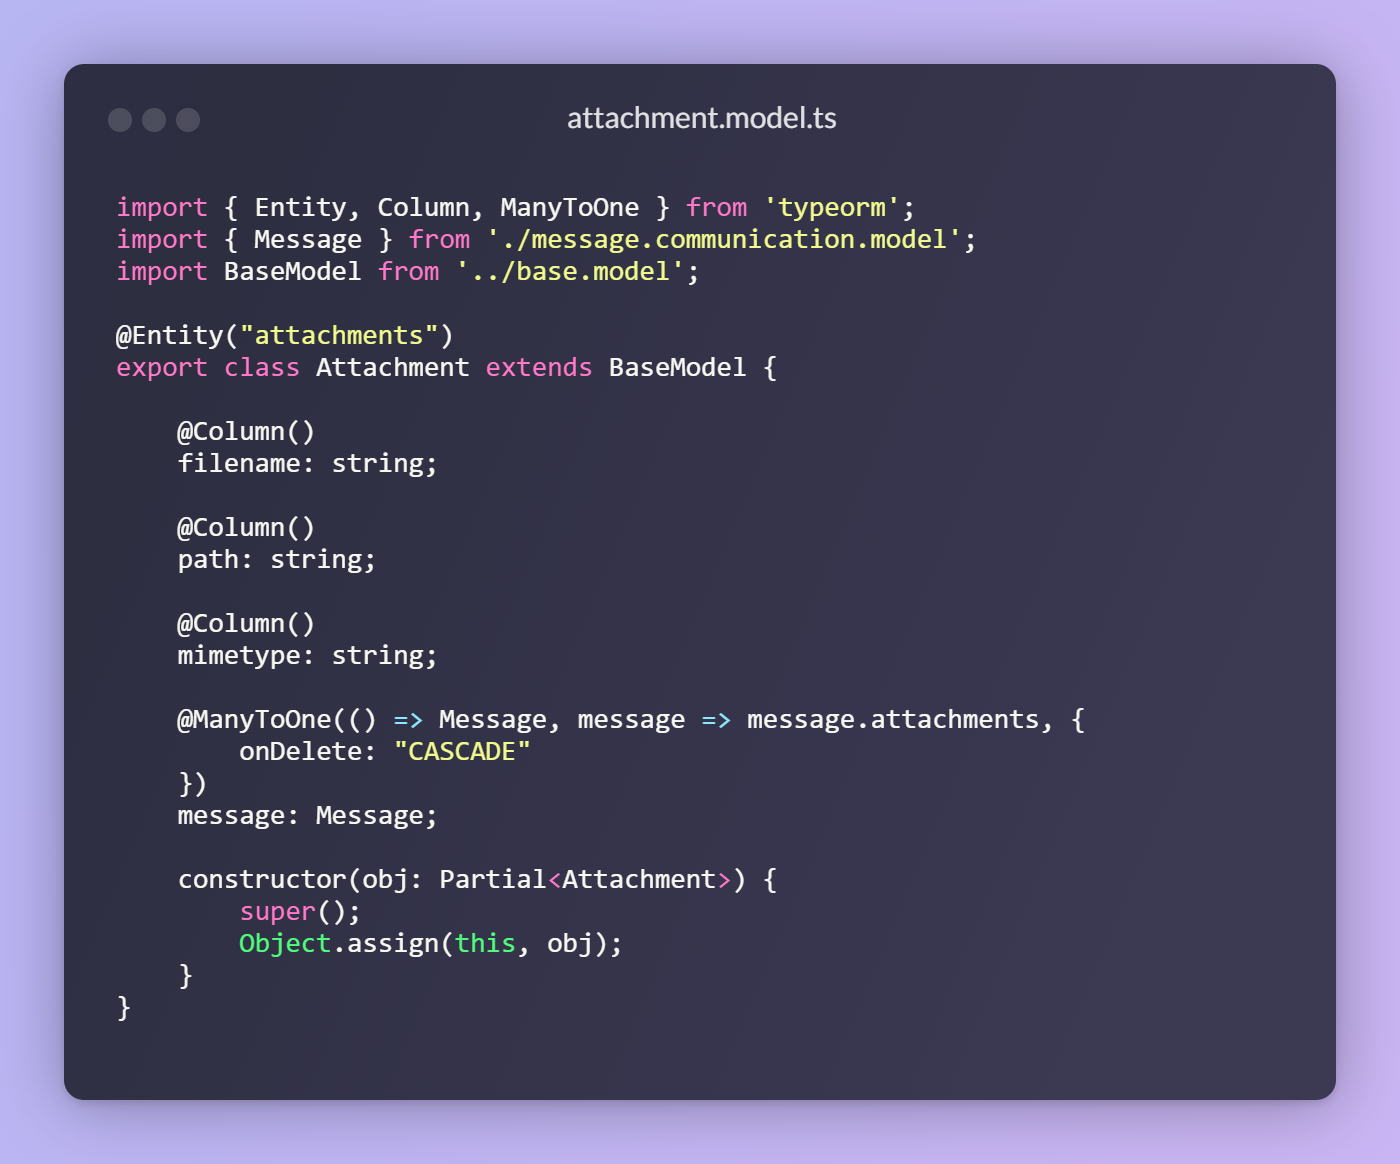
\includegraphics[width=16cm]{assets/annexes/snippet.png}
    \caption{Code pour implémenter la classe attachement avec Typeorm}
\end{figure}

\begin{figure}[H]
    \centering
    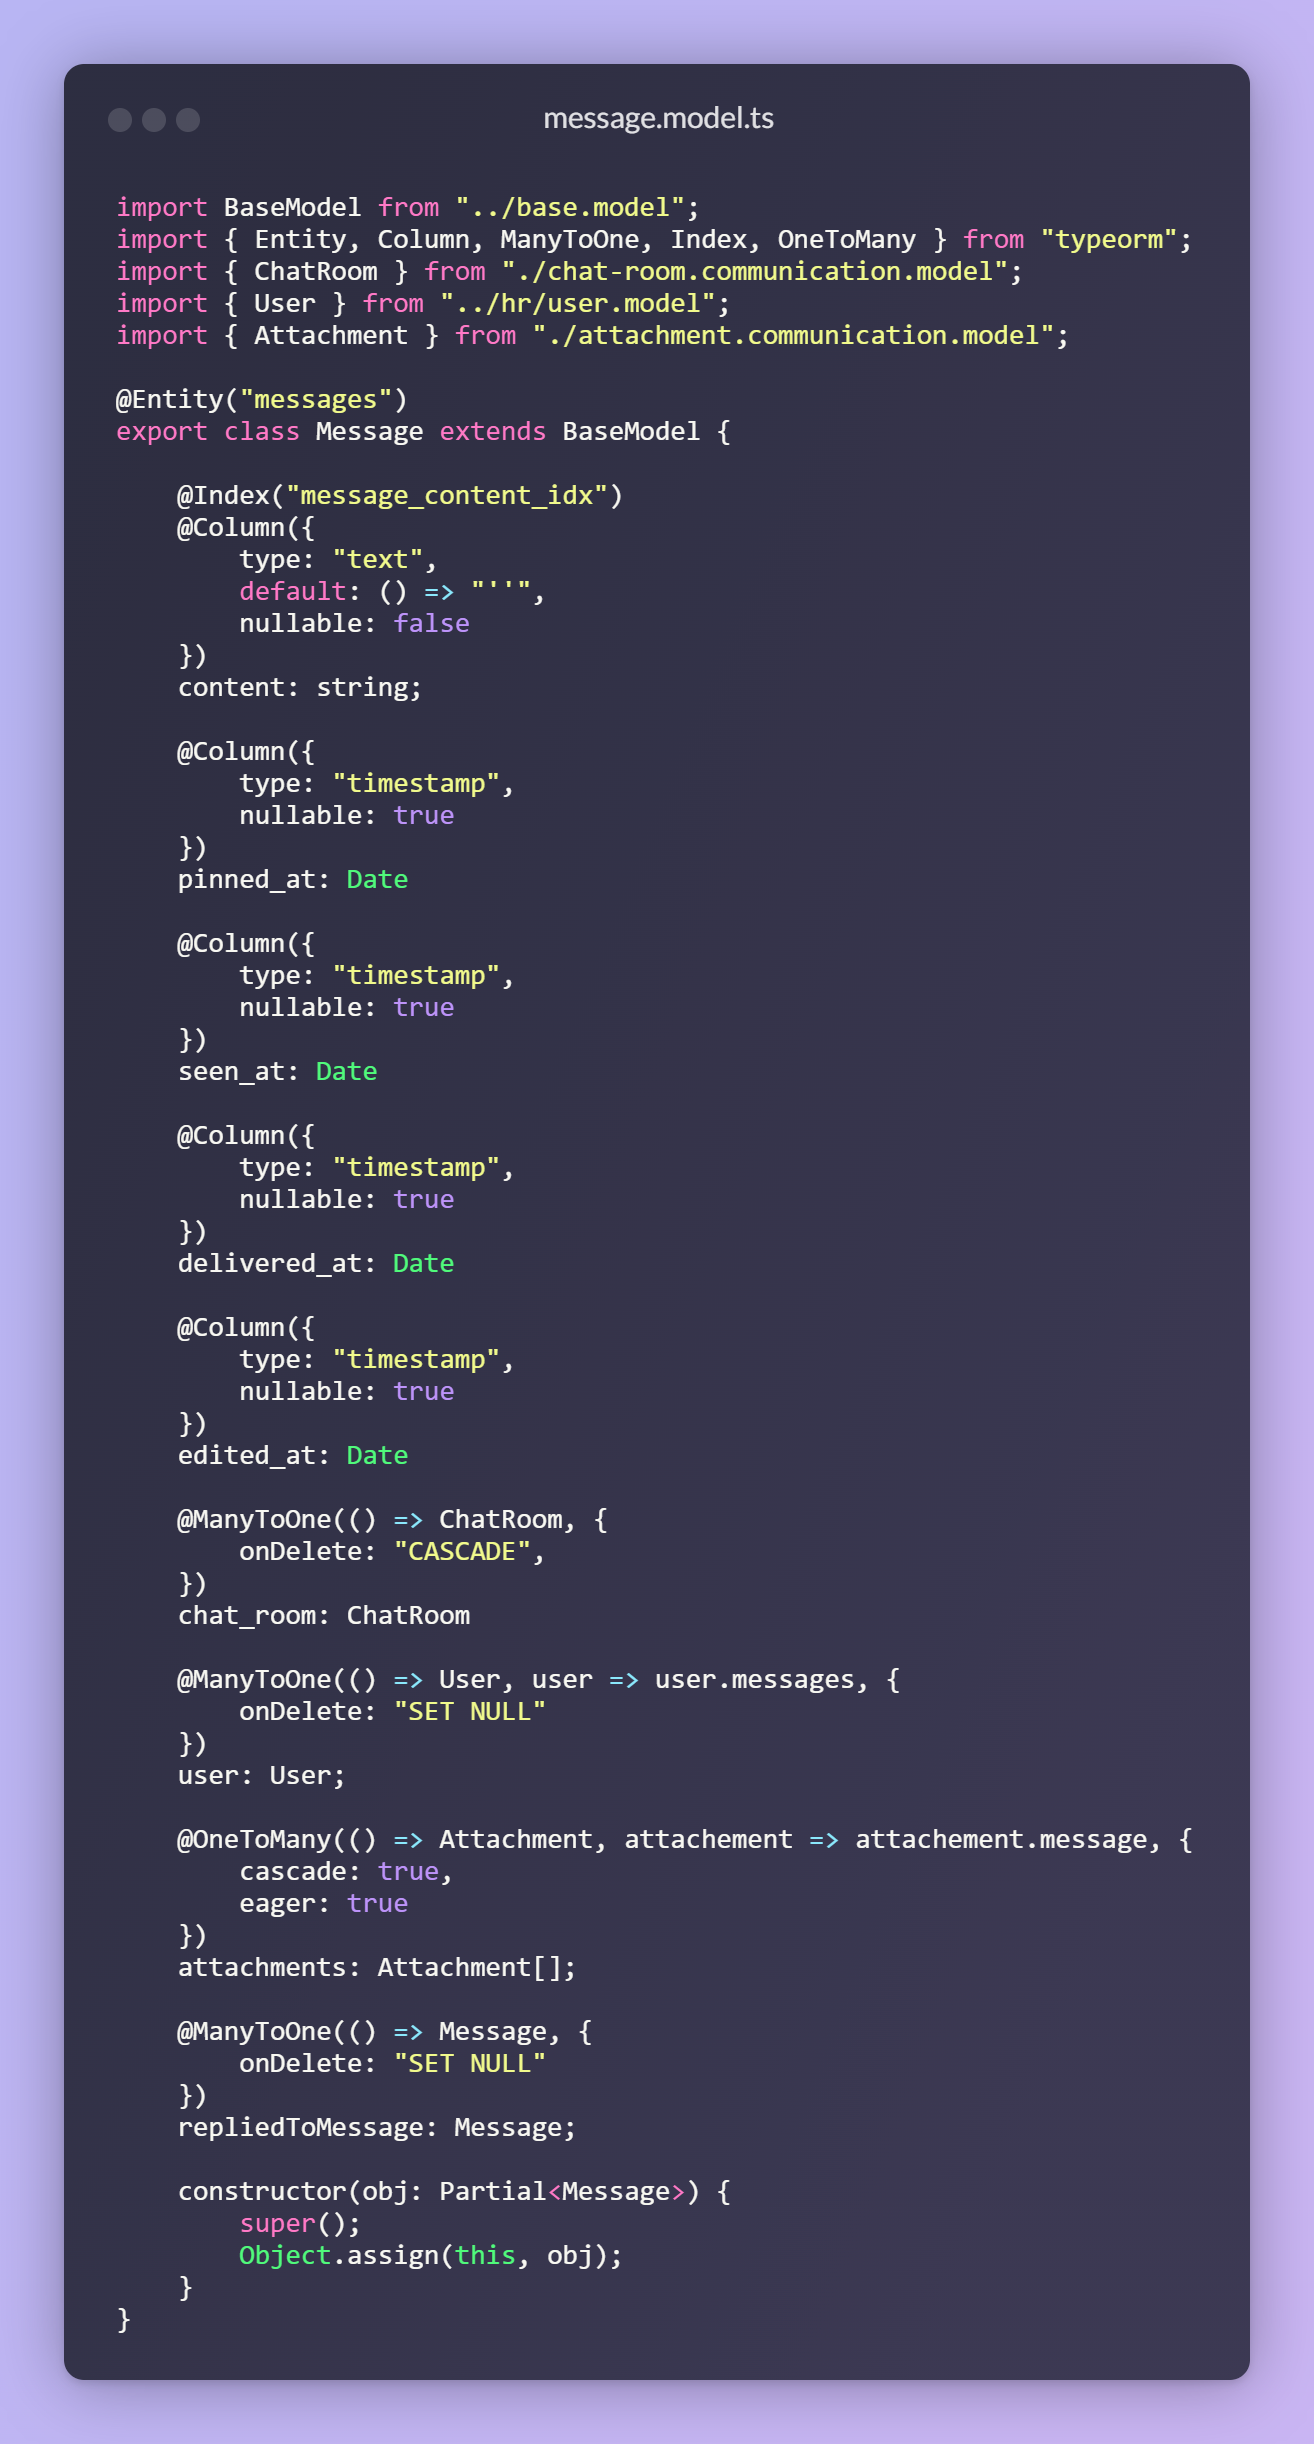
\includegraphics[width=13.5cm]{assets/annexes/snippet (1).png}
    \caption{Code pour implémenter la classe message avec Typeorm}
\end{figure}

\begin{figure}[H]
    \centering
    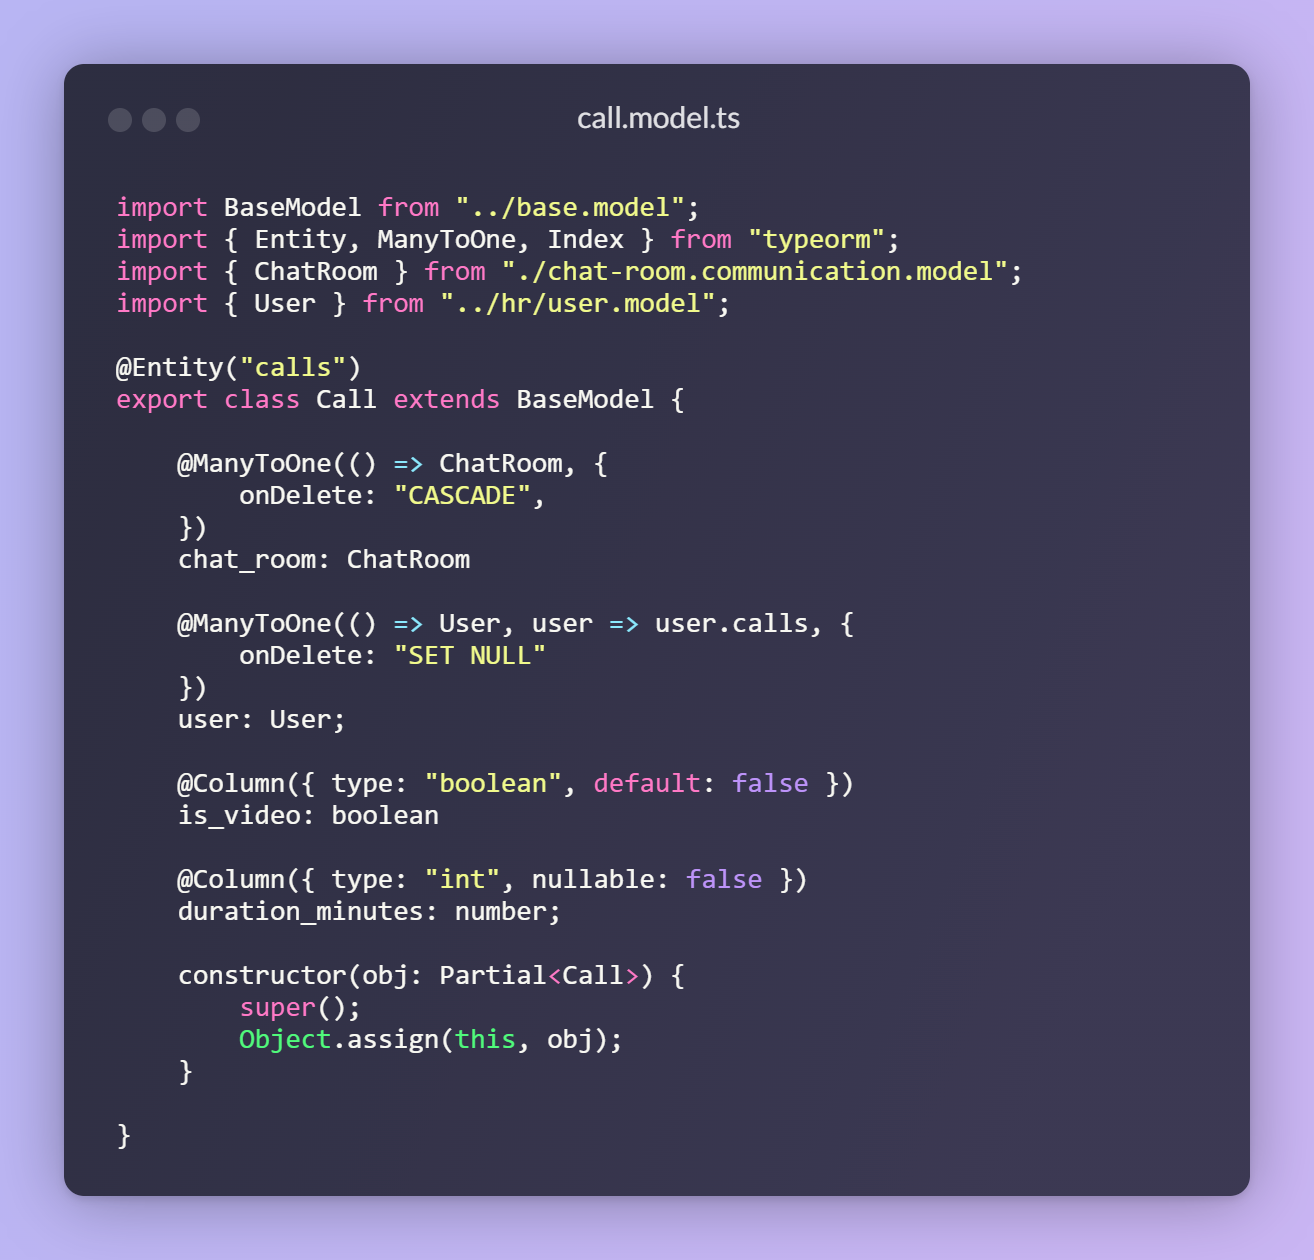
\includegraphics[width=16cm]{assets/annexes/snippet (2).png}
    \caption{Code pour implémenter la classe call avec Typeorm}
\end{figure}

\begin{figure}[H]
    \centering
    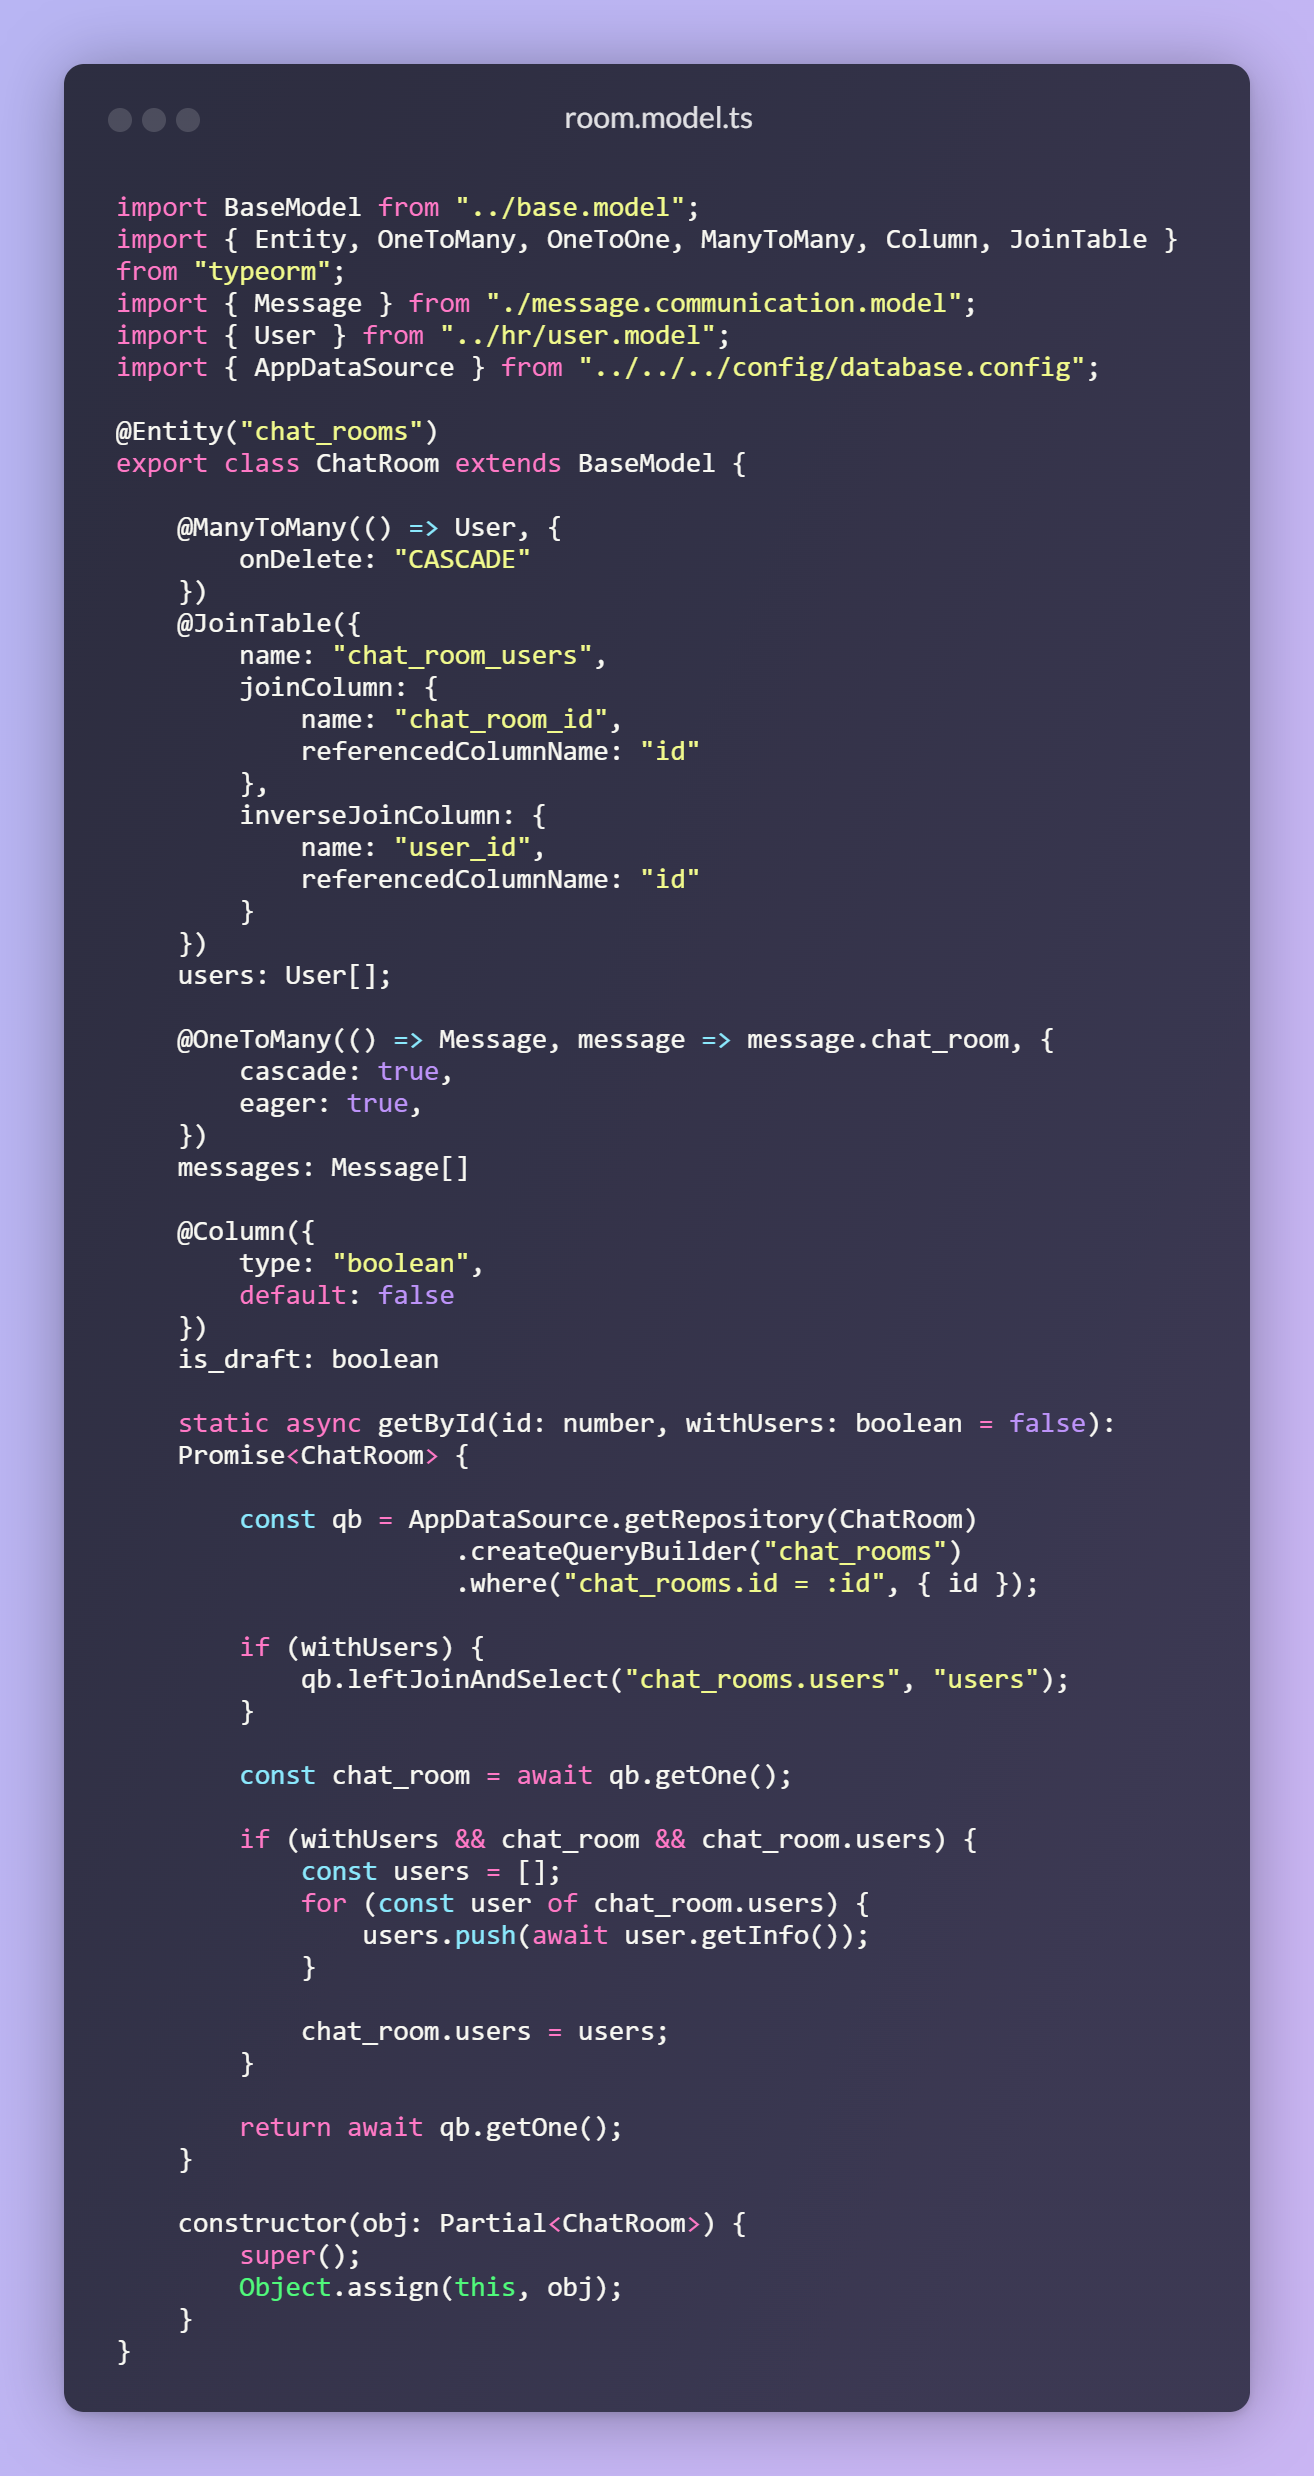
\includegraphics[width=13.5cm]{assets/annexes/snippet (3).png}
    \caption{Code pour implémenter la classe room avec Typeorm}
\end{figure}

\clearpage

Après avoir implémenté le modèle, la prochaine étape consiste à développer les services qui utiliseront ces modèles. Dans ce projet, nous avons mis en place deux classes de services essentielles.

\begin{description}
    \item[- Service de gestion des salons (RoomService)] : Cette classe contient trois méthodes principales :
        \begin{enumerate}
            \item \verb|findChatRooms| : récupère tous les salons de discussion associés à l'utilisateur qui effectue la requête.
            \item \verb|findOrCreateChatRoom| : recherche un salon existant entre deux utilisateurs ou en crée un nouveau si aucun n'existe.
            \item \verb|addMessage| : ajoute un message à un salon de discussion existant.
        \end{enumerate}
        
    \item[- Service de gestion des messages (\textbf{MessageService})] : Ce service gère l'envoi et la récupération des messages dans une conversation :
        \begin{enumerate}
            \item \verb|findByChatRoomId| : récupère tous les messages d'un salon de discussion donné, en incluant les informations des utilisateurs, rôles et pièces jointes.
            \item \verb|newMessage| : crée un nouveau message en associant l'utilisateur, le salon de discussion et les éventuelles pièces jointes.
        \end{enumerate}
\end{description}

\vspace{0.35cm}

Après avoir implémenté ces services, on peut désormais passer à l'implémentation de la classe responsable des connexions instantannées. 

\vspace{0.35cm}

Commençons d'abord à initialiser la classe. 

\clearpage

\begin{figure}[H]
    \centering
    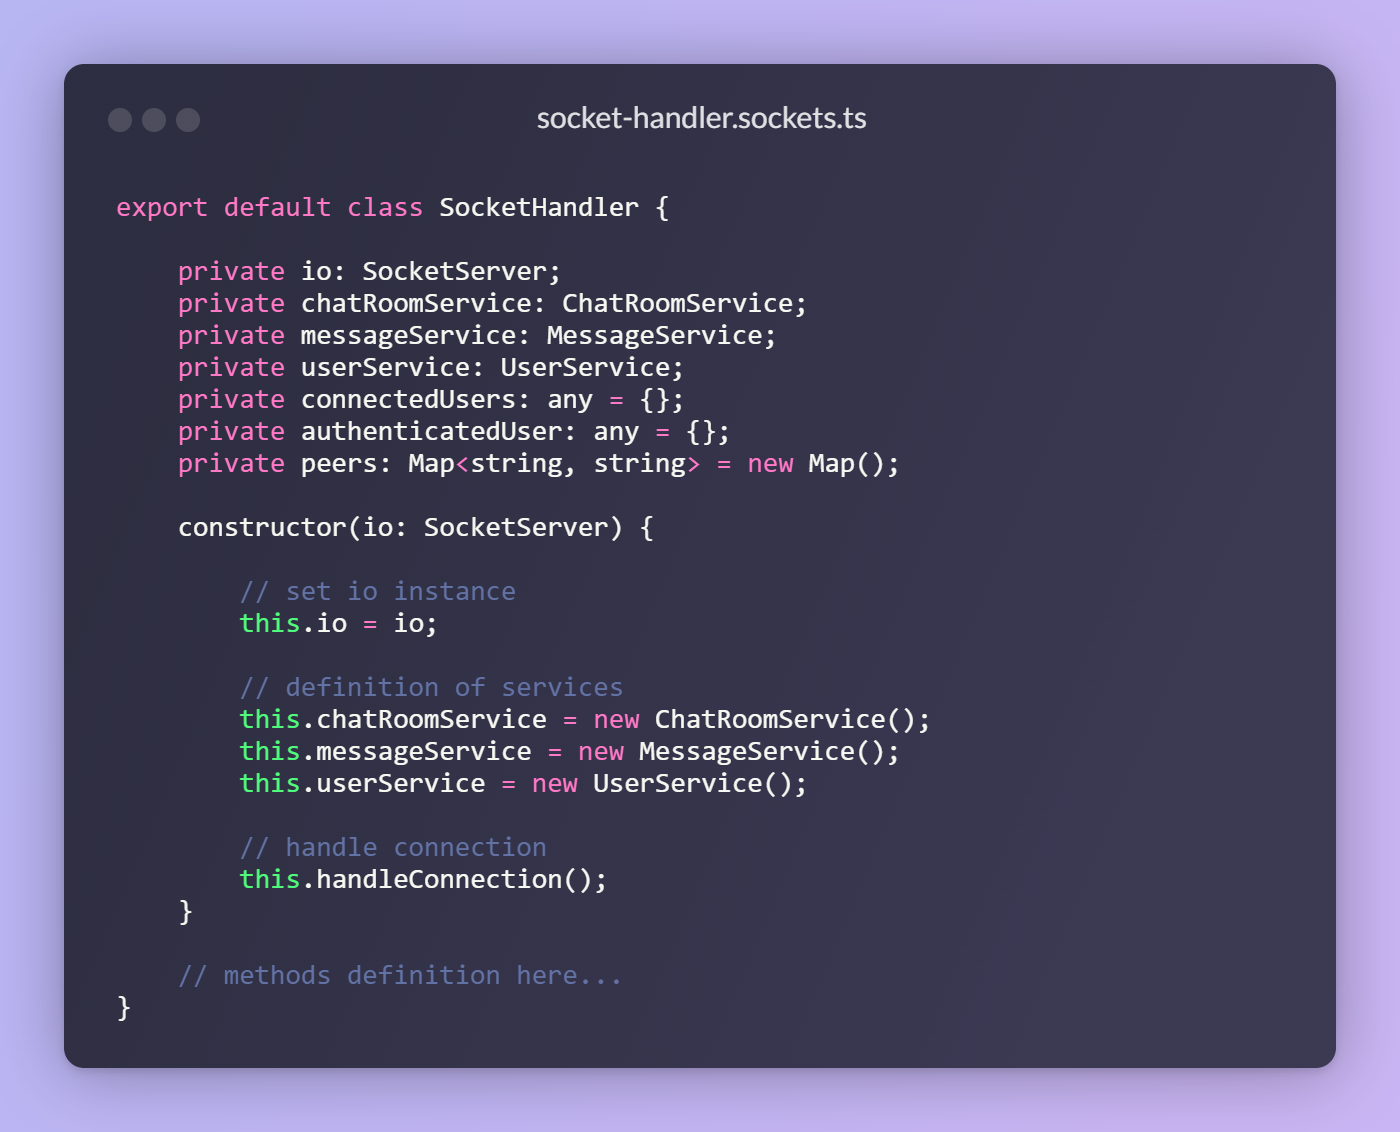
\includegraphics[width=16cm]{assets/annexes/snippet (4).png}
    \caption{Socket Handler - Définition de la classe et du constructeur}
\end{figure}

\vspace{1cm}

Ensuite, nous devons définir la méthode responsable de gérer la connexion du socket. Cette méthode vérifie si l'utilisateur est authentifié puis elle monte les évenements avec les différents handlers de chaque évenement. 
Elle charge ensuite la liste des salons ou conversations concernant l'utilisateur et la retourne grâce à un évenement émis.

\begin{figure}[H]
    \centering
    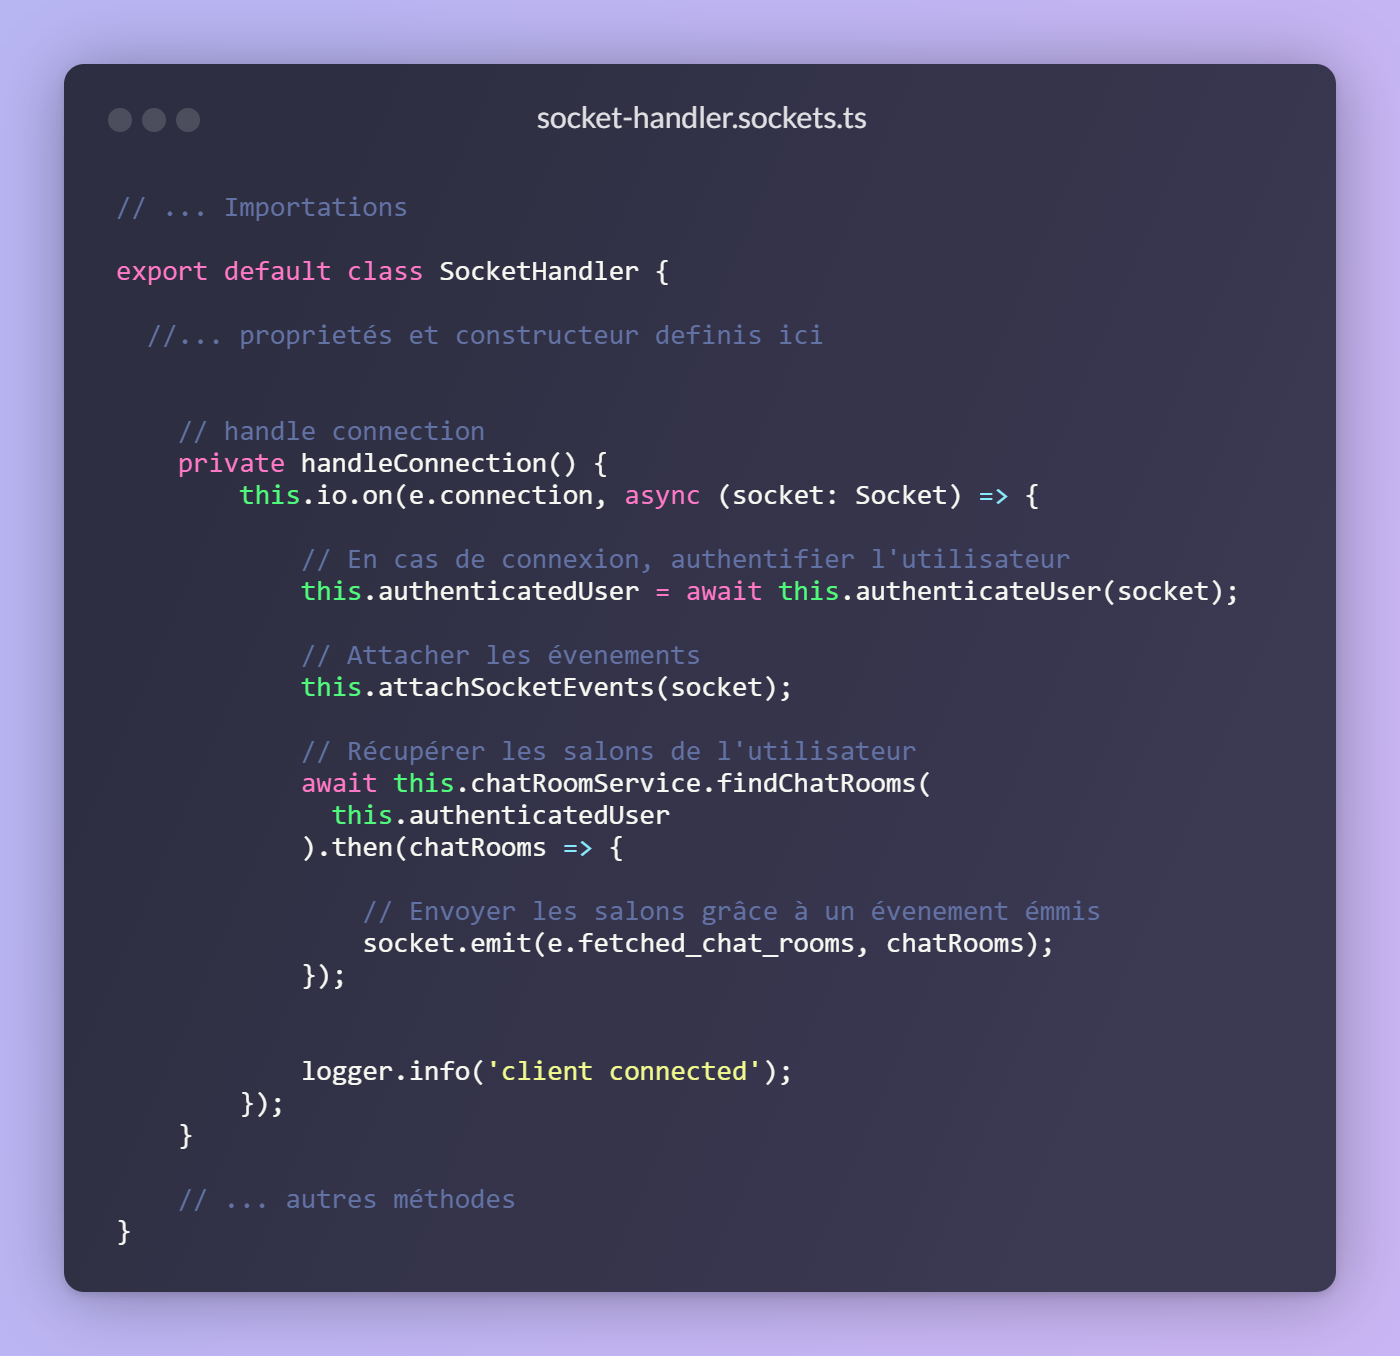
\includegraphics[width=16cm]{assets/annexes/snippet (5).png}
    \caption{Socket Handler - Gestionnaire de Connexions}
\end{figure}

\vspace{1cm}

Après nous allons définir la méthode responsable de vérifier l'authentification des requêtes puis définir la fonction (\verb|attachSocketEvents| qui monte les évenements avec les différents handlers de chaque évenements. La dernière étape sera de définir les différents handlers des évenements écoutés par notre serveur socket.

\begin{figure}[H]
    \centering
    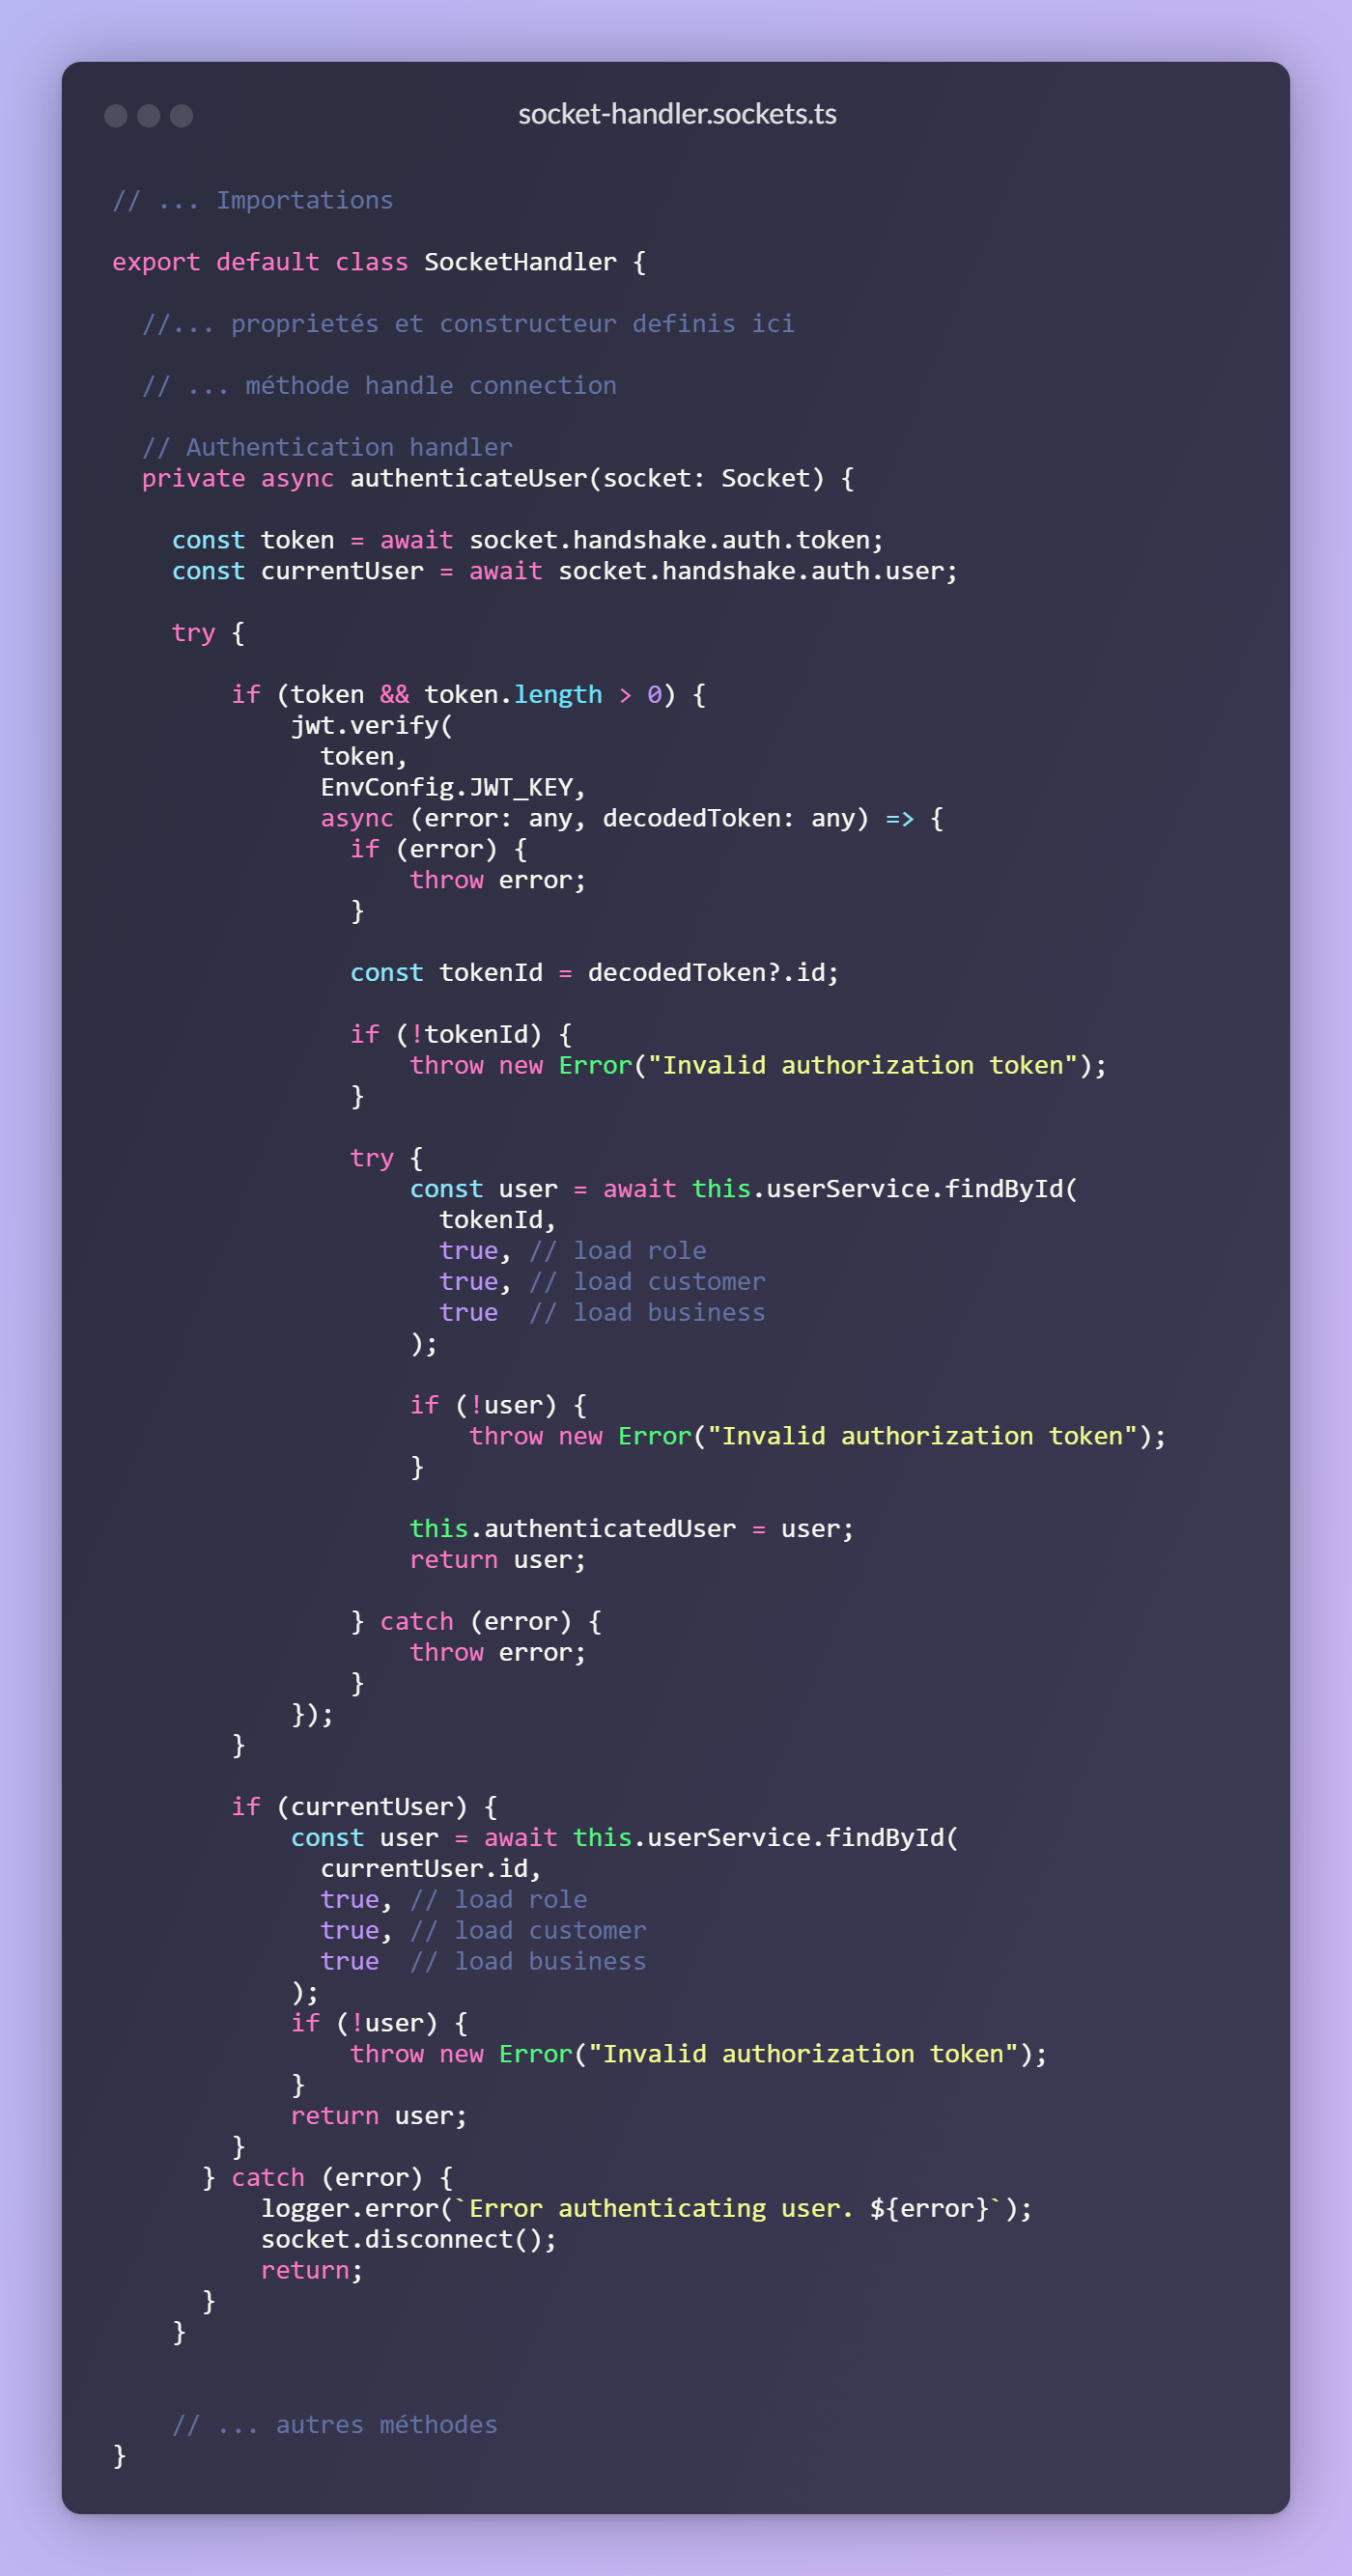
\includegraphics[width=13cm]{assets/annexes/snippet (6).png}
    \caption{Socket Handler - Middleware d'authentification }
\end{figure}

\vspace{1cm}

\begin{figure}[H]
    \centering
    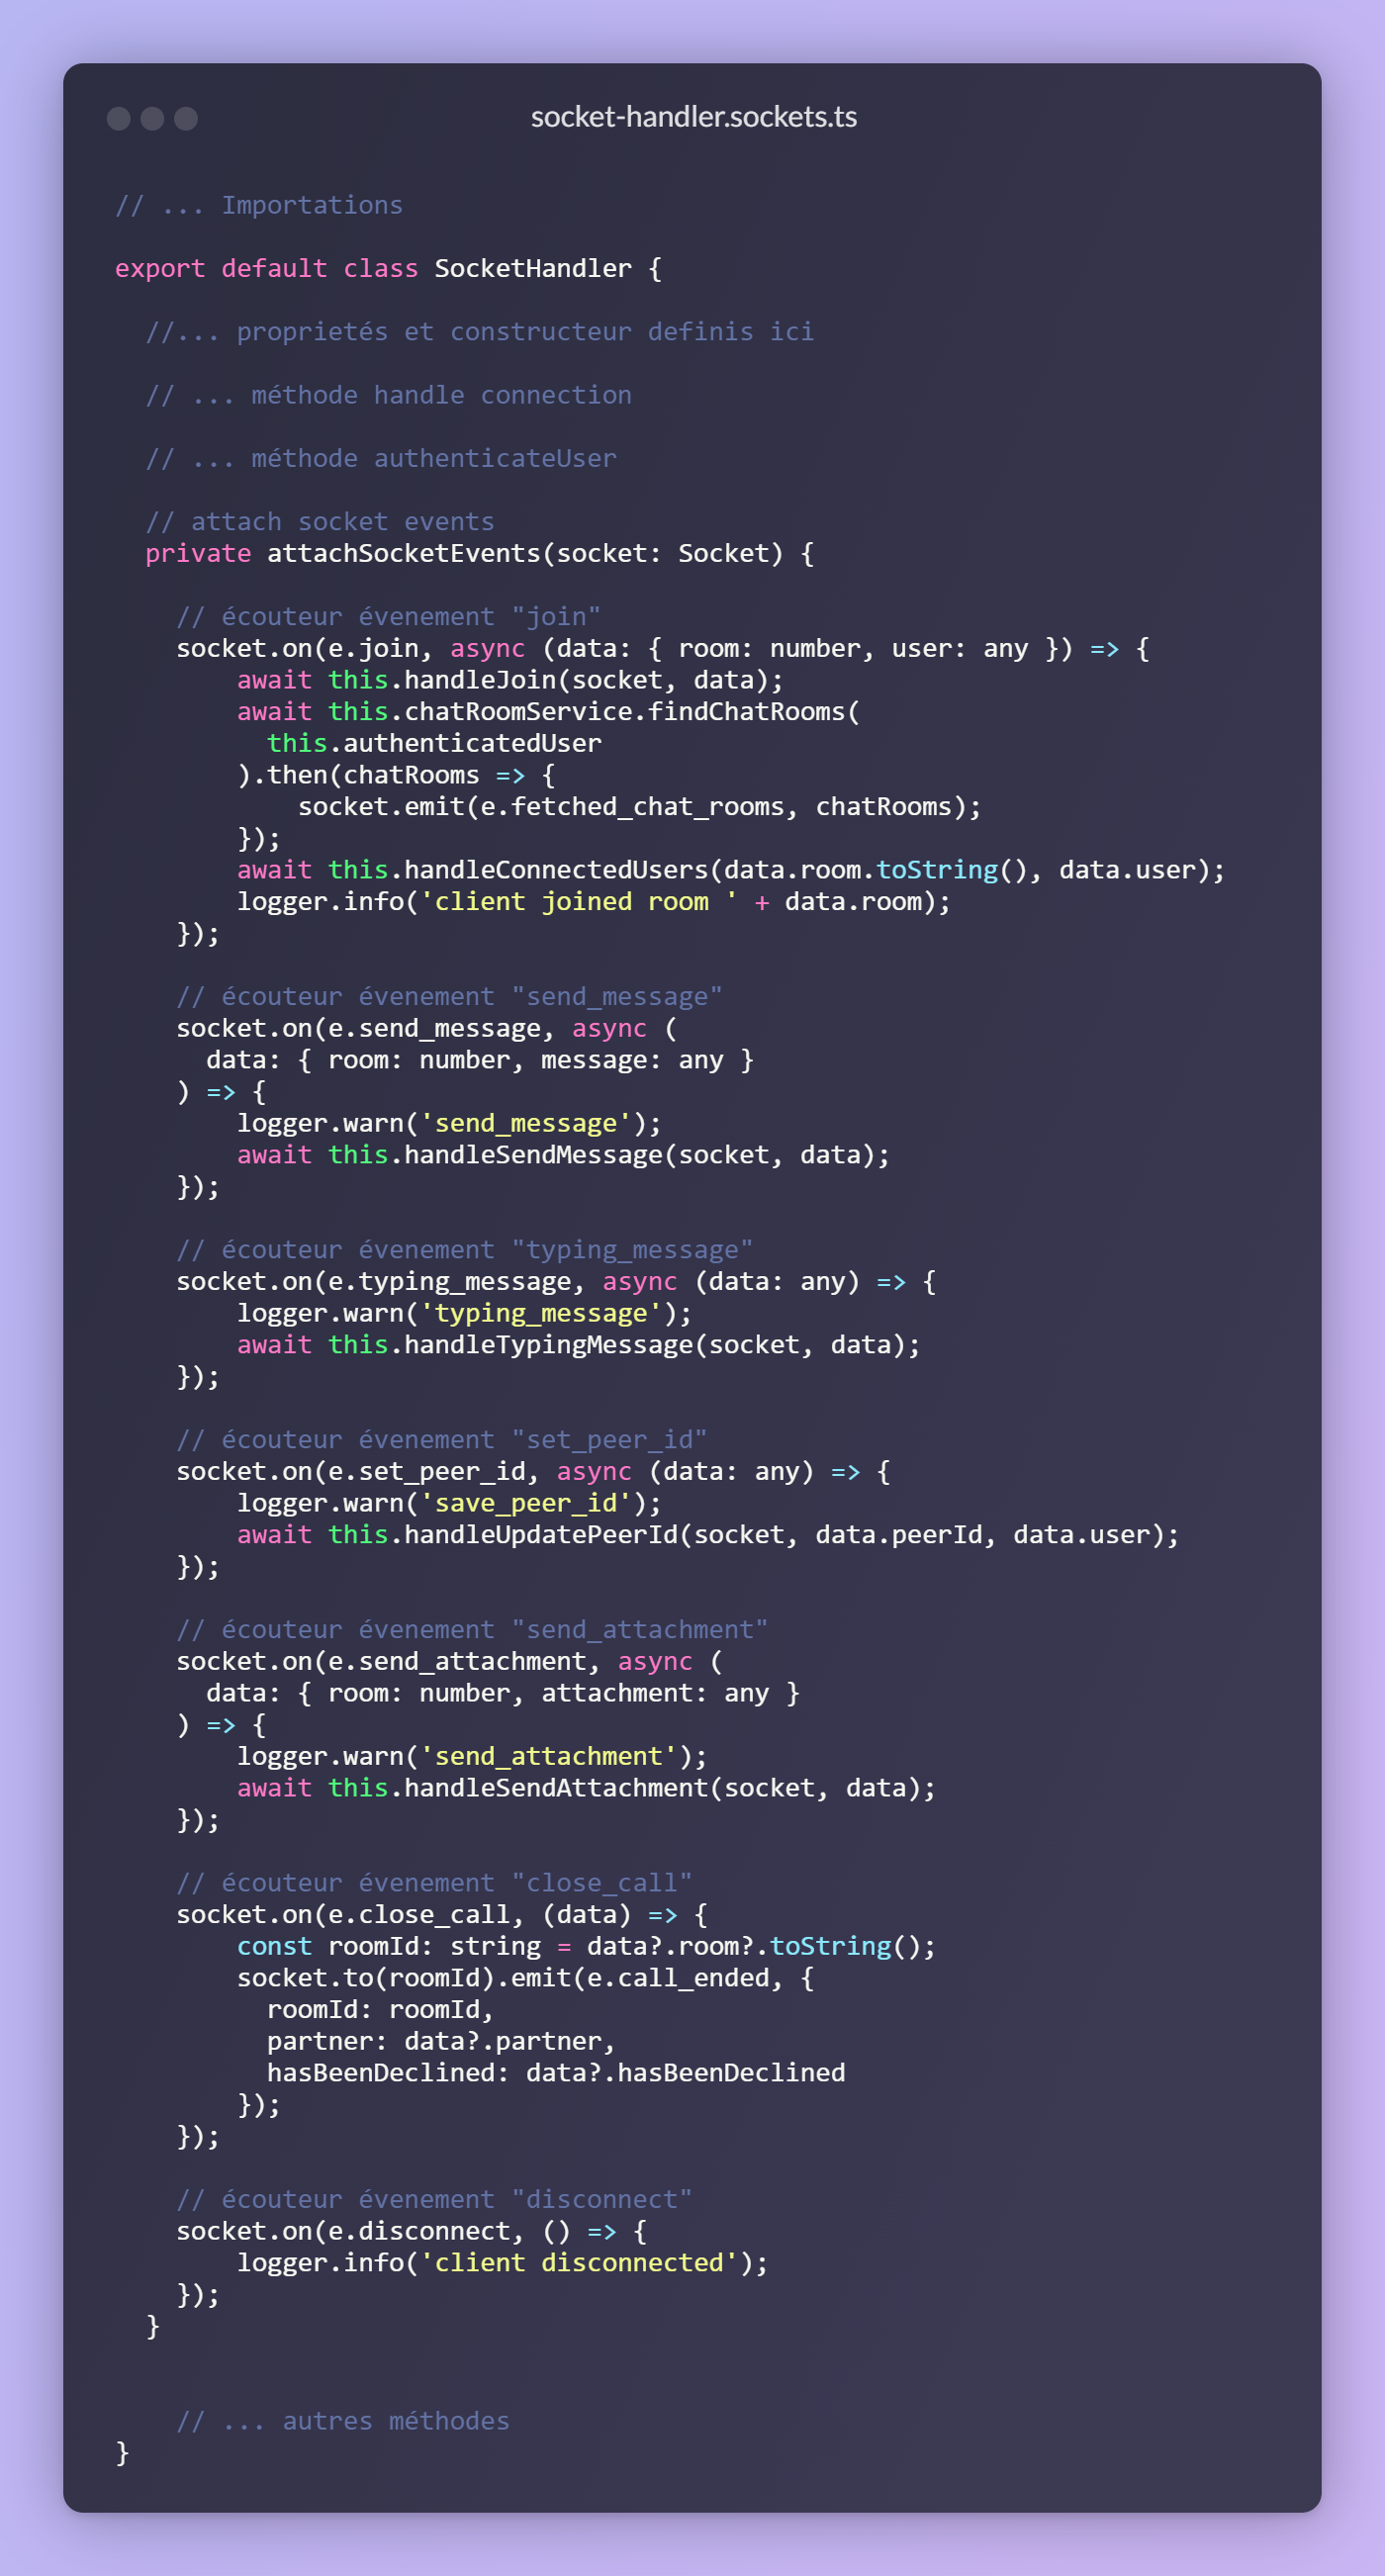
\includegraphics[width=13cm]{assets/annexes/snippet (7).png}
    \caption{Socket Handler - Fonction AttachSocketEvents}
\end{figure}

\vspace{1cm}

\begin{figure}[htp]
  \centering
  \subfloat{\label{fig:first}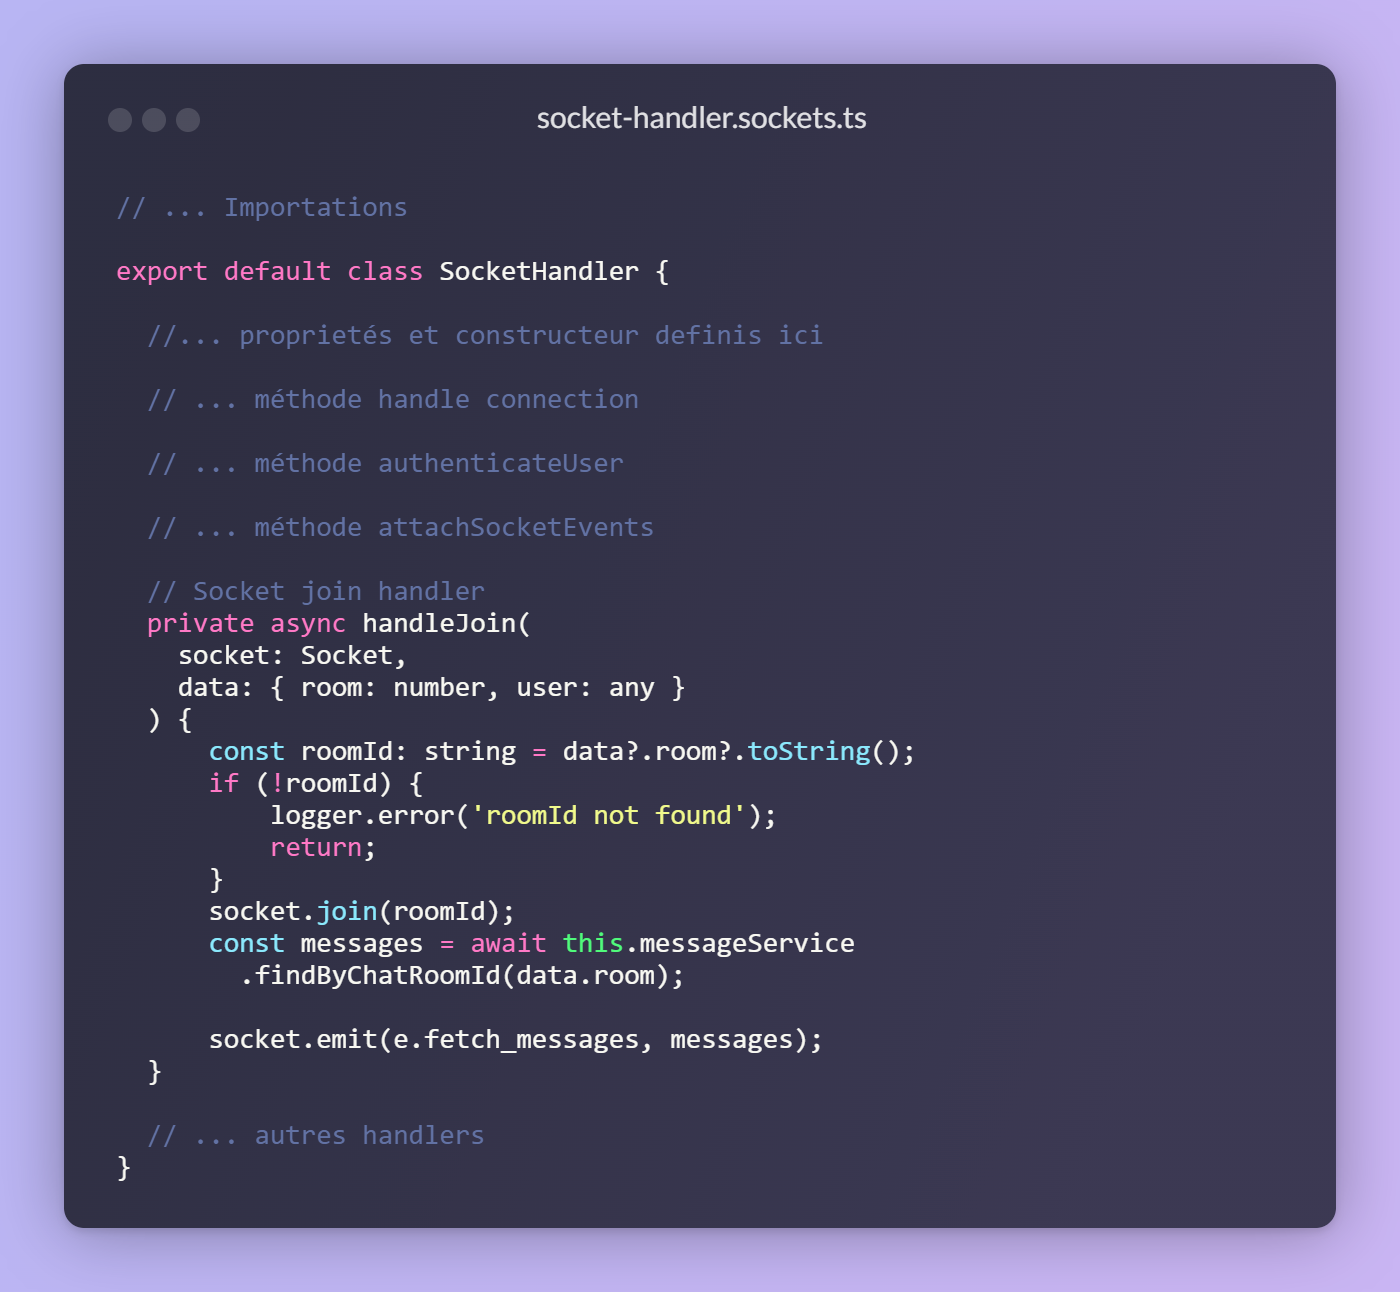
\includegraphics[width=7.3cm, height=10.7cm]{assets/annexes/snippet (9).png}}
  ~
  \subfloat{\label{fig:second}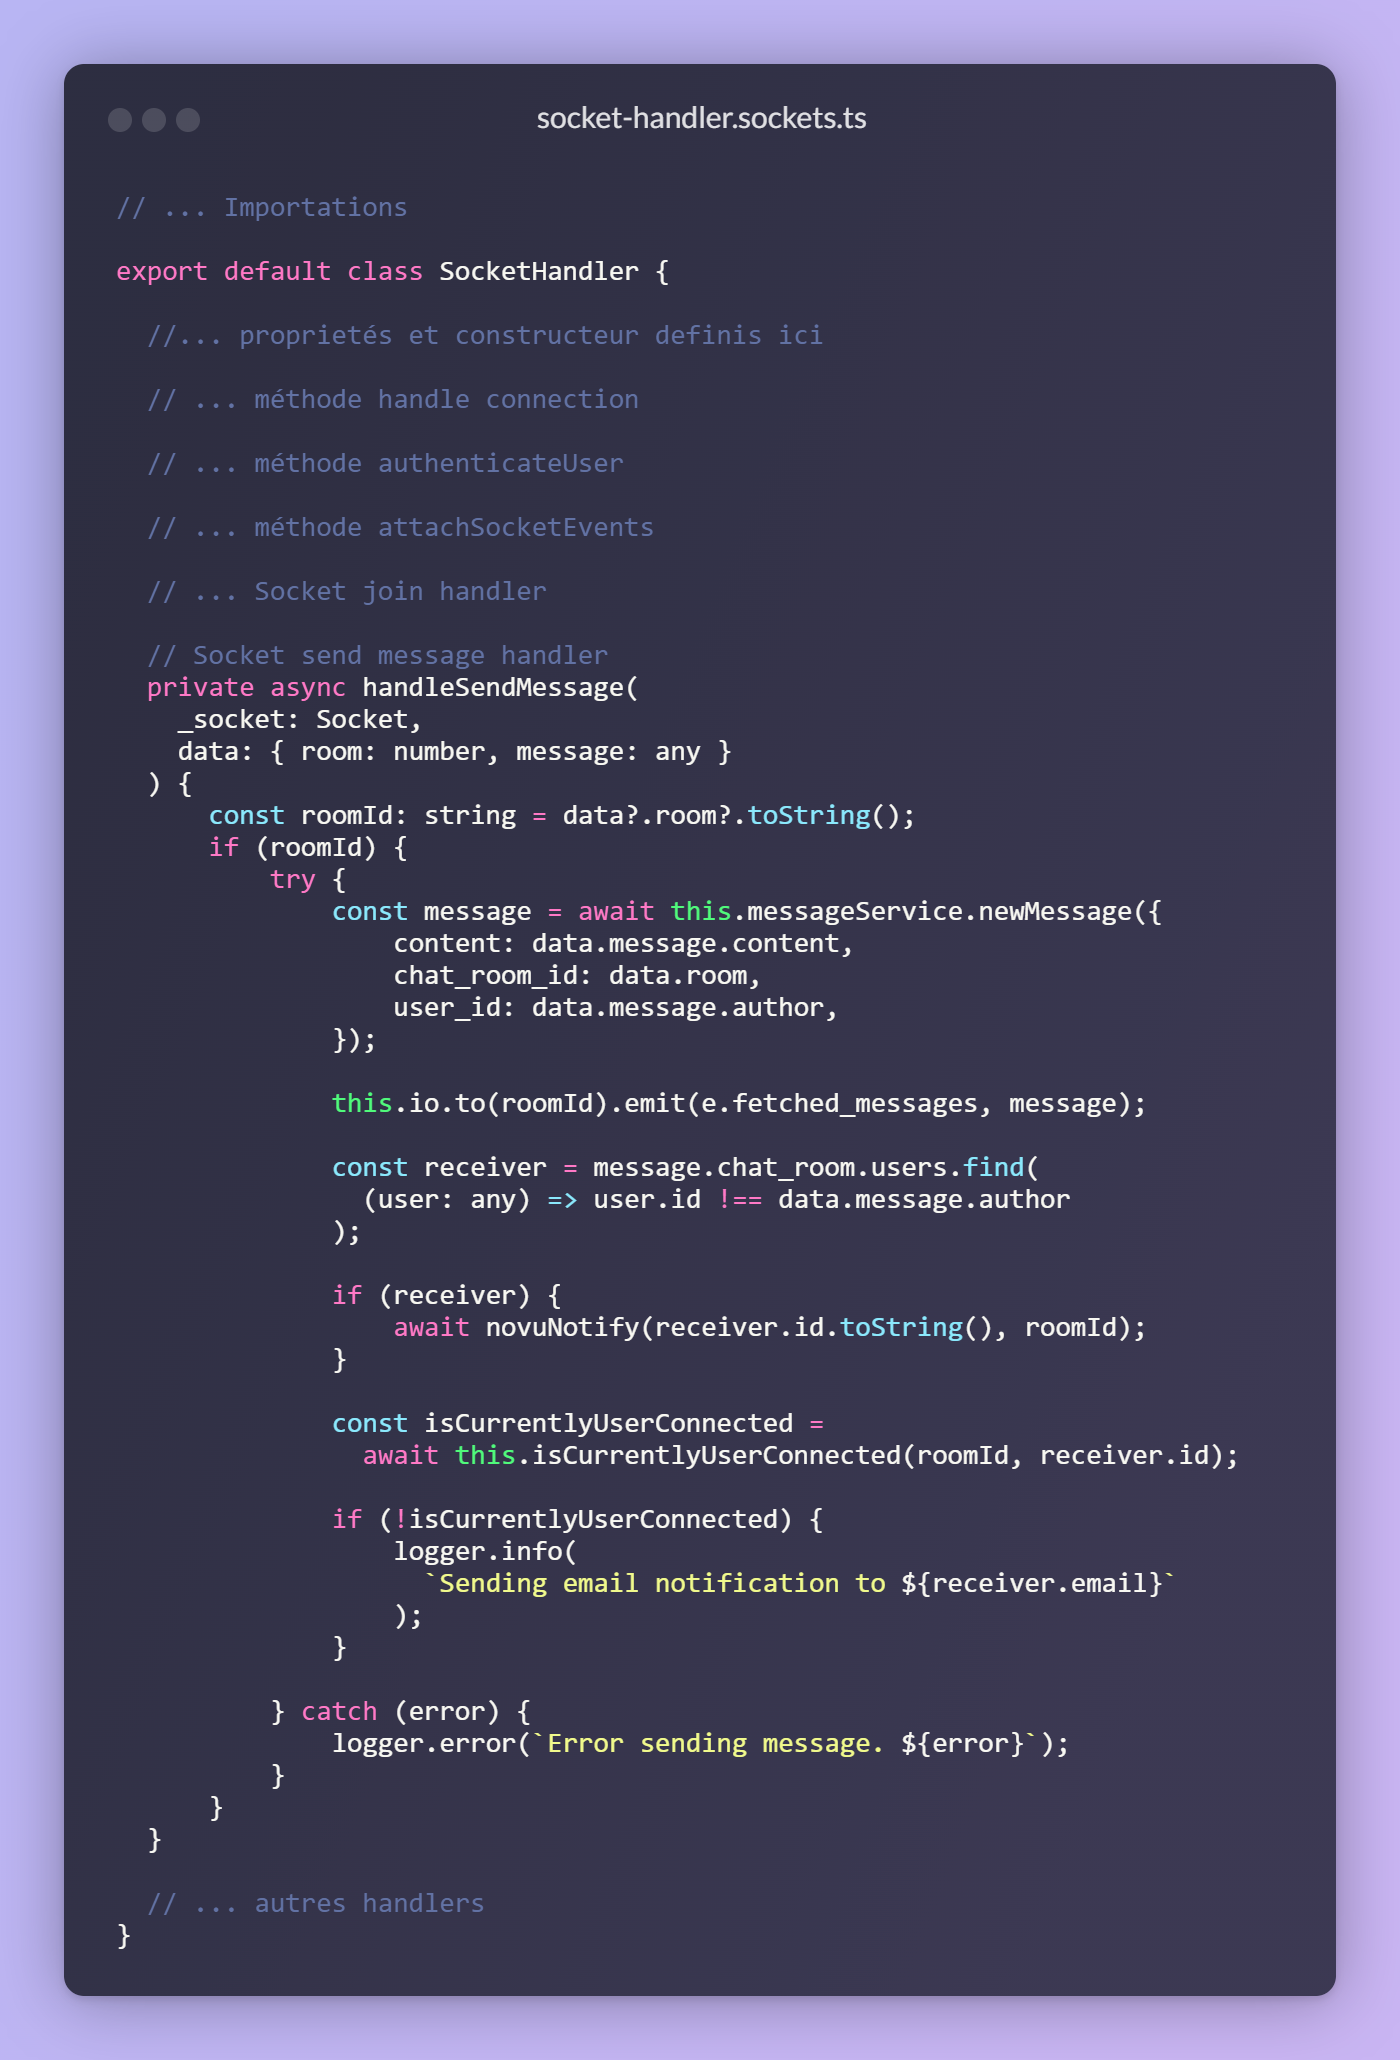
\includegraphics[width=7.3cm]{assets/annexes/snippet (10).png}}
  ~\\
    \subfloat{\label{fig:third}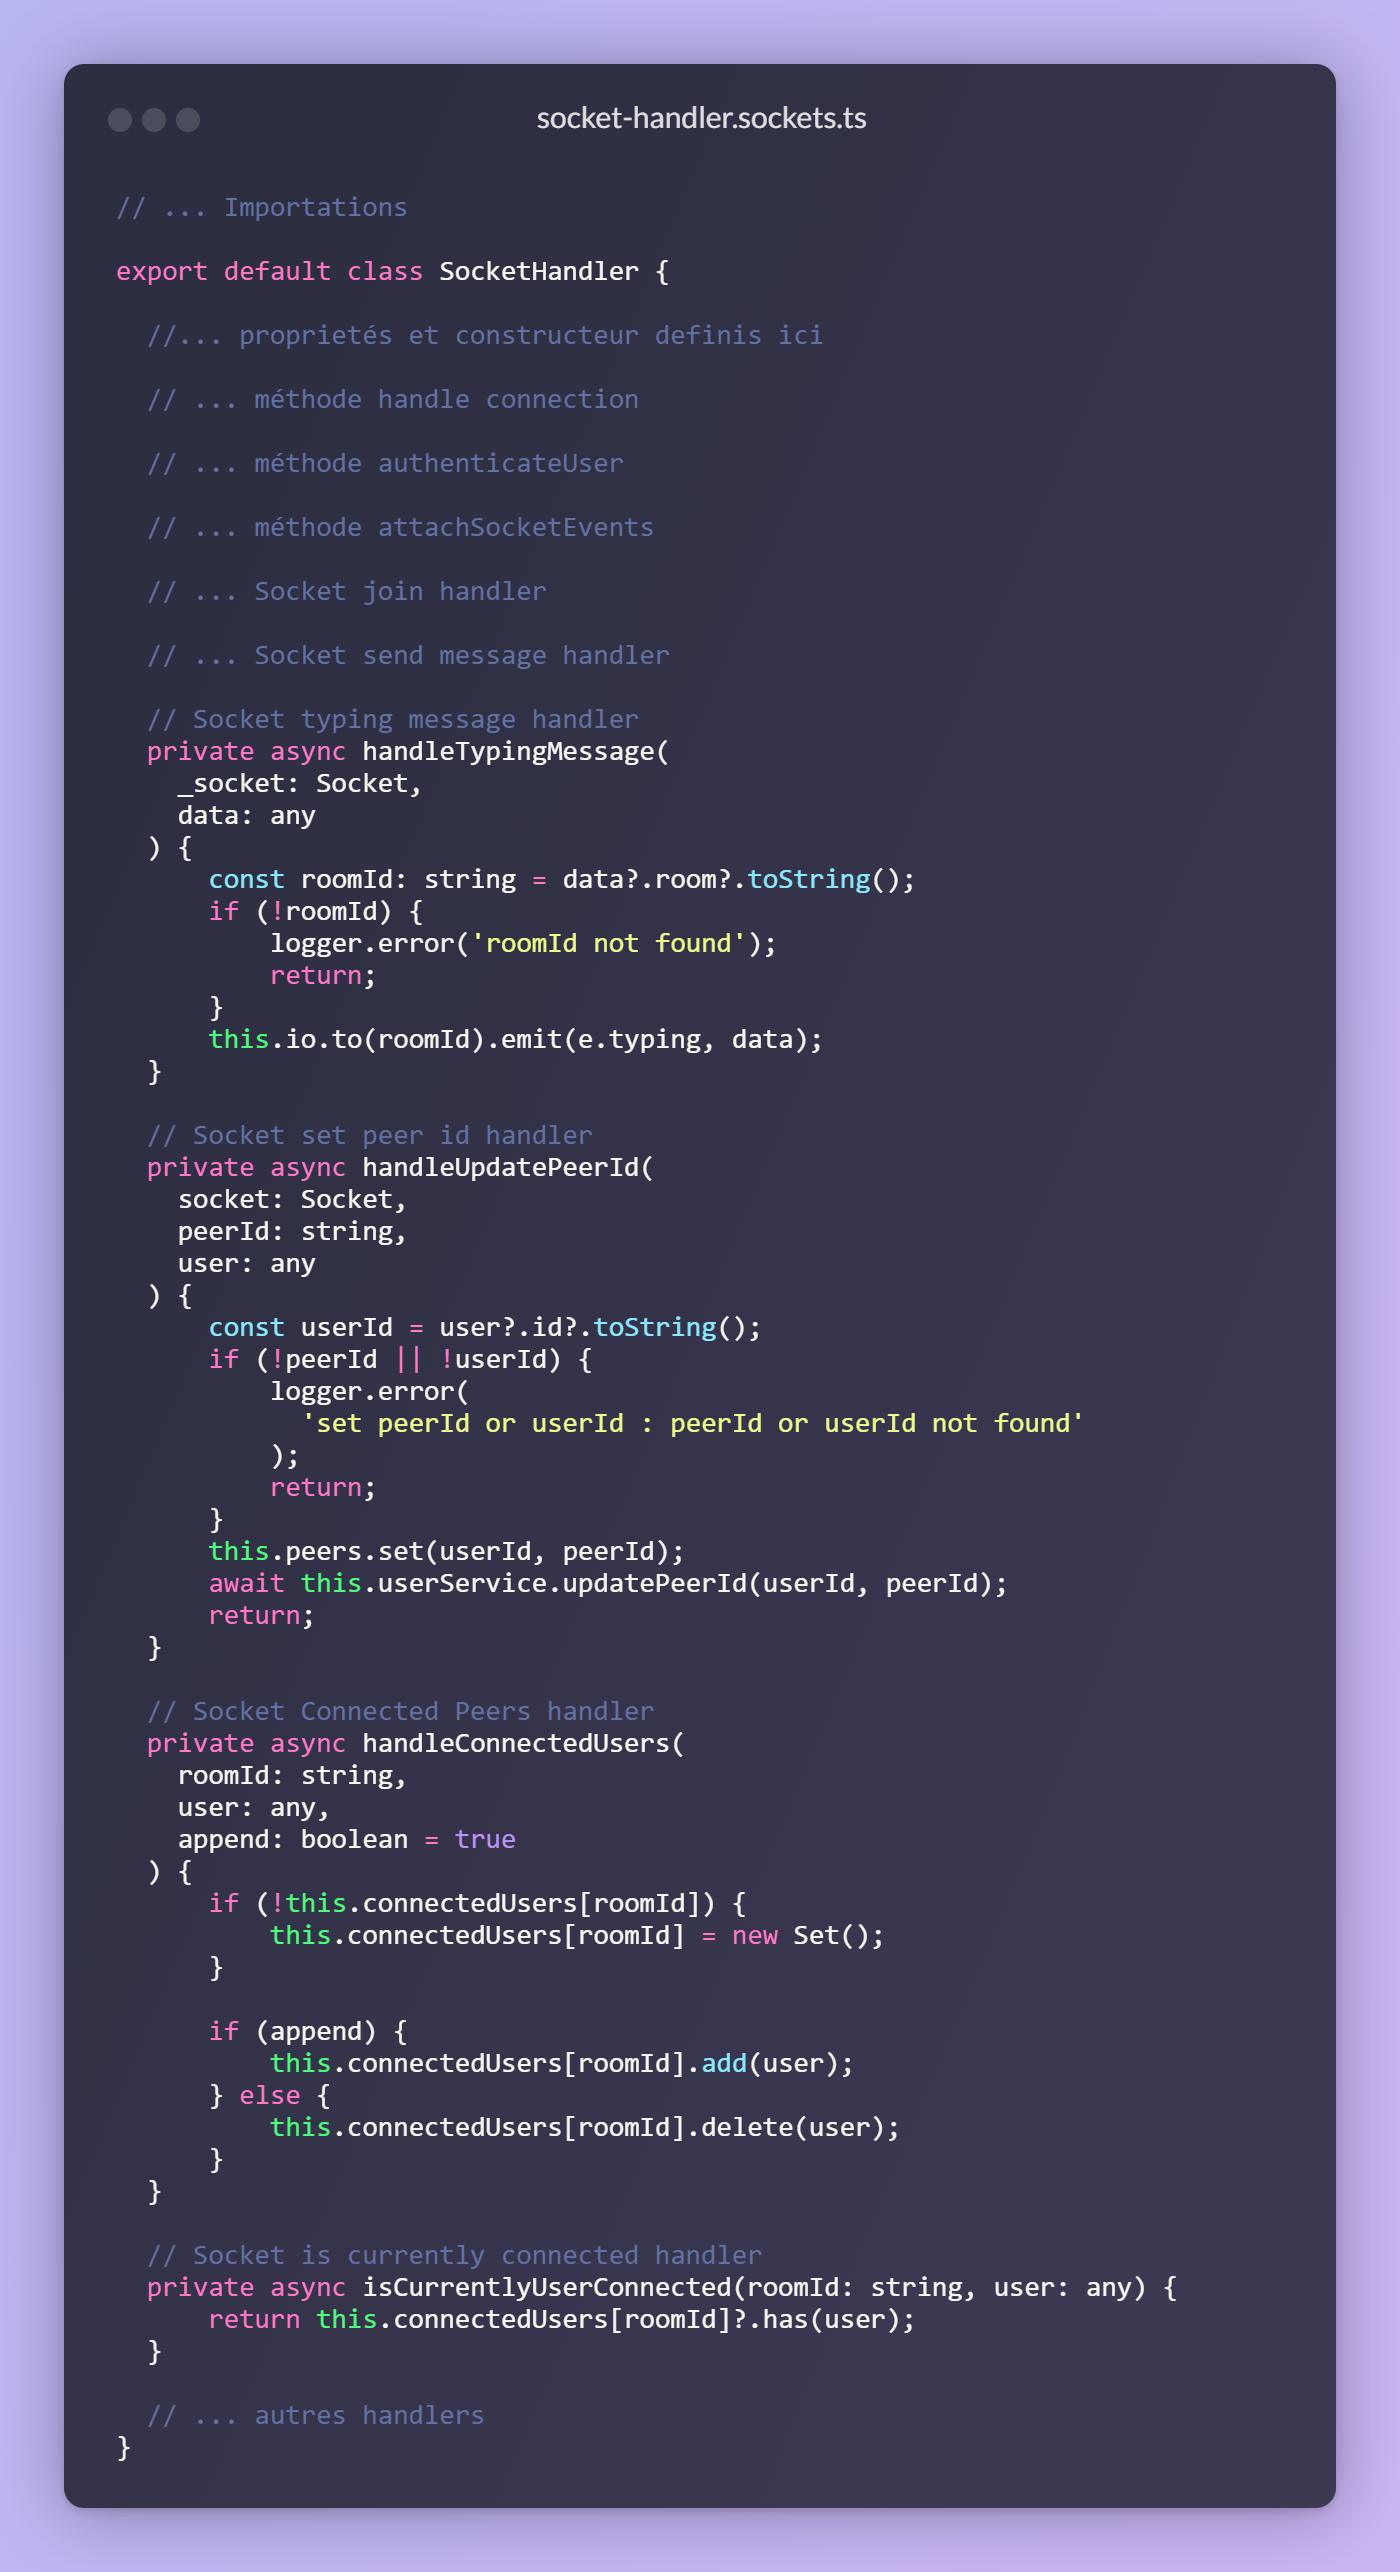
\includegraphics[width=7.3cm]{assets/annexes/snippet (11).png}}
  ~
  \subfloat{\label{fig:fourth}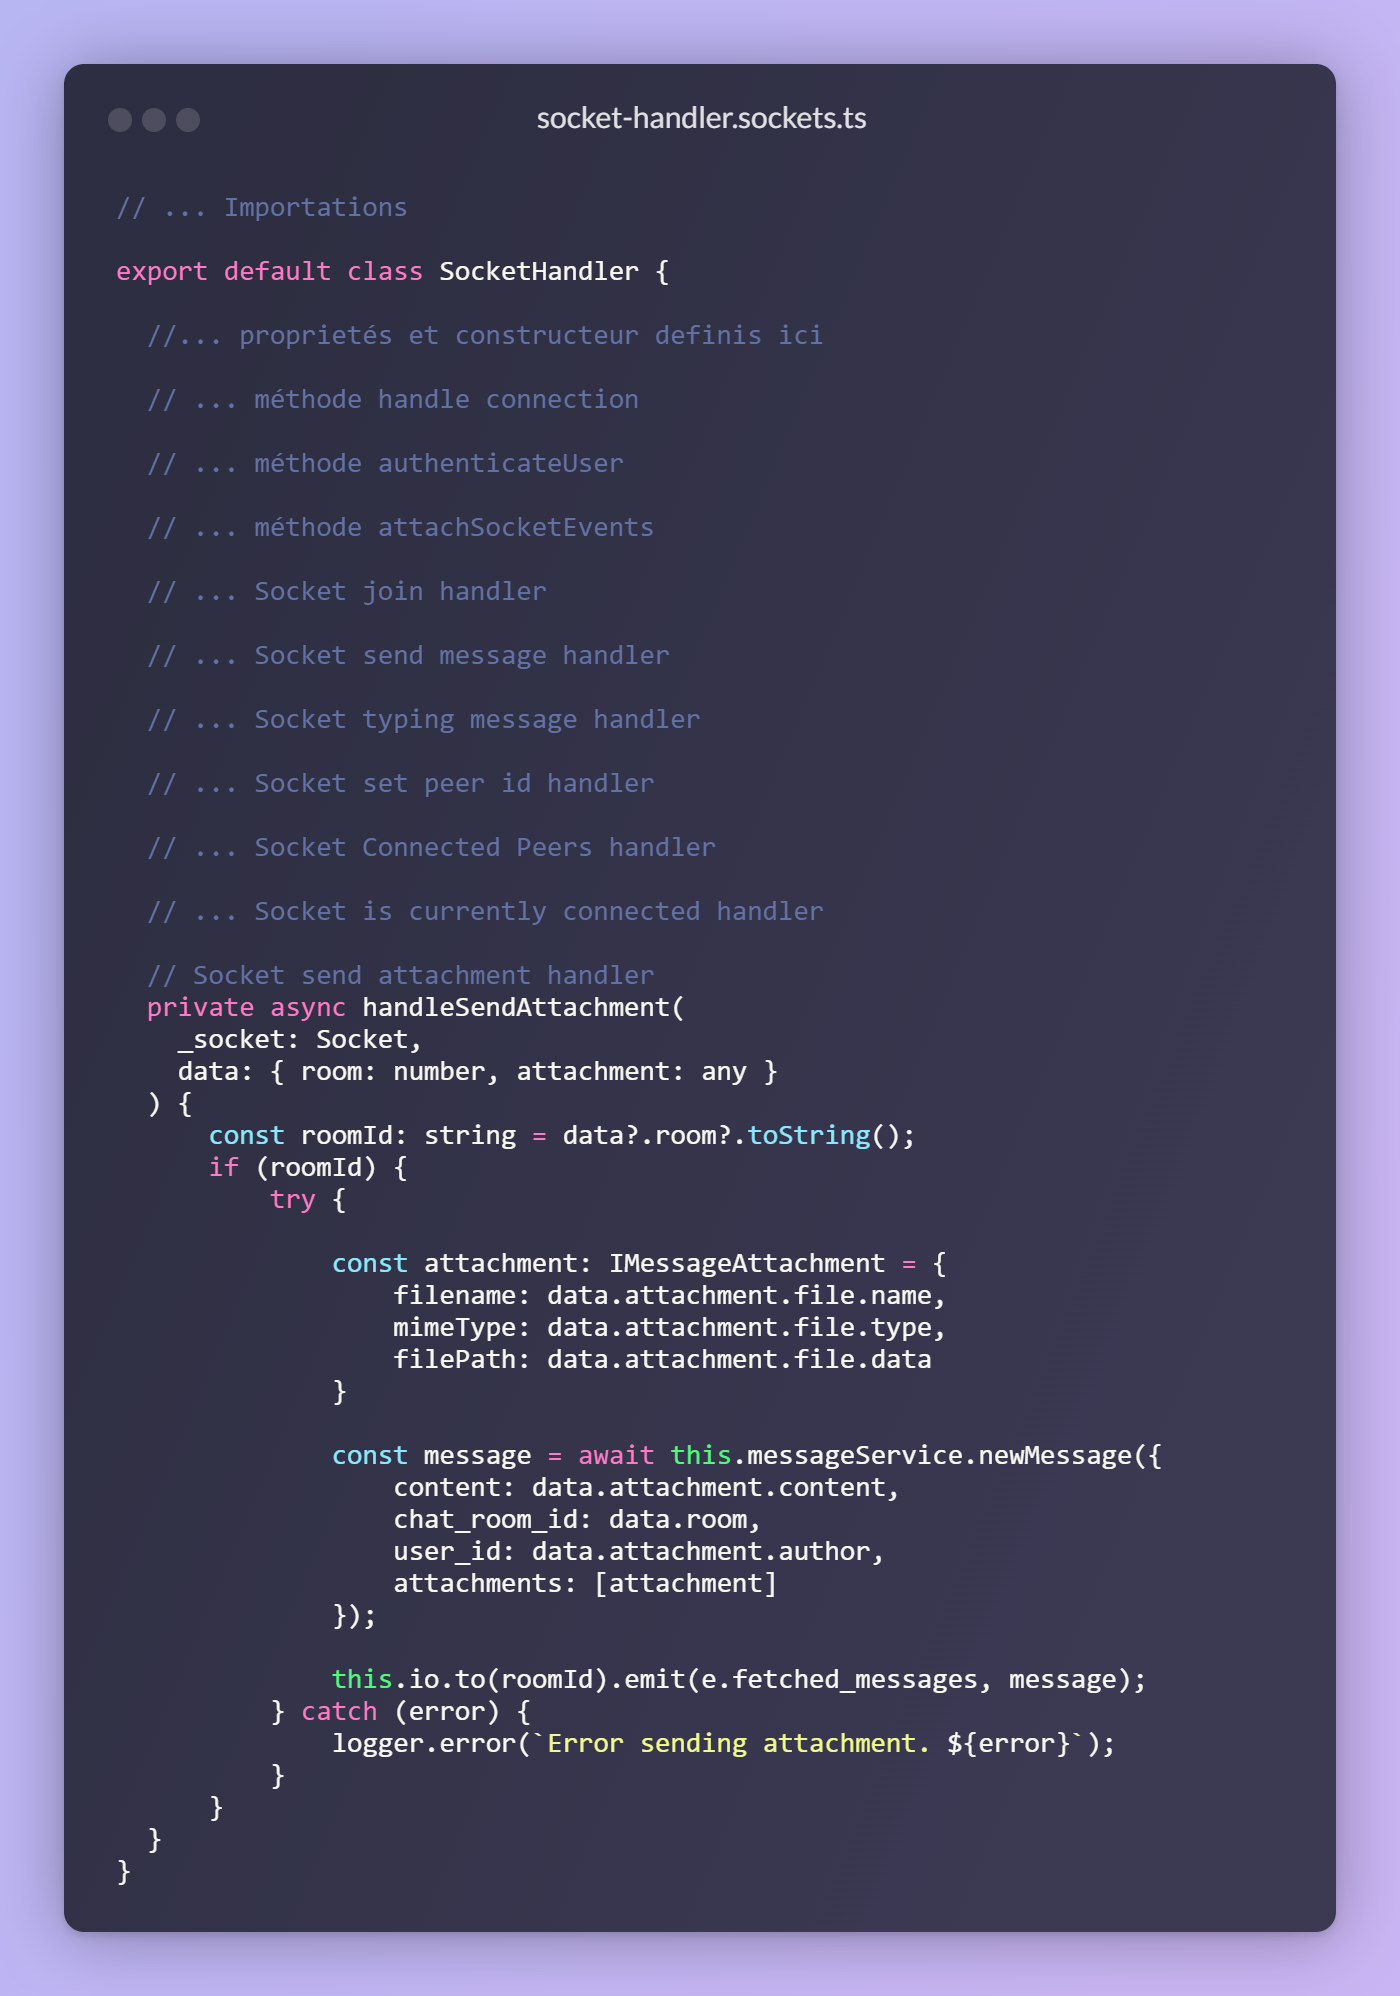
\includegraphics[width=7.3cm, height=13.4cm]{assets/annexes/snippet (12).png}}
  \caption{Socket Handler - Fonctions Handlers}
  \label{fig:gallerieSockets}
\end{figure}

\clearpage

\vspace{1cm}

Une fois que cette classe est implémentée, nous devons la monter dans le point d'entrée de l'application (\verb|app.bootstrap.ts|.). Ci-dessous un exemple du code du fichier \verb|app.bootstrap.ts|

\vspace{0.35cm}

\begin{figure}[H]
    \centering
    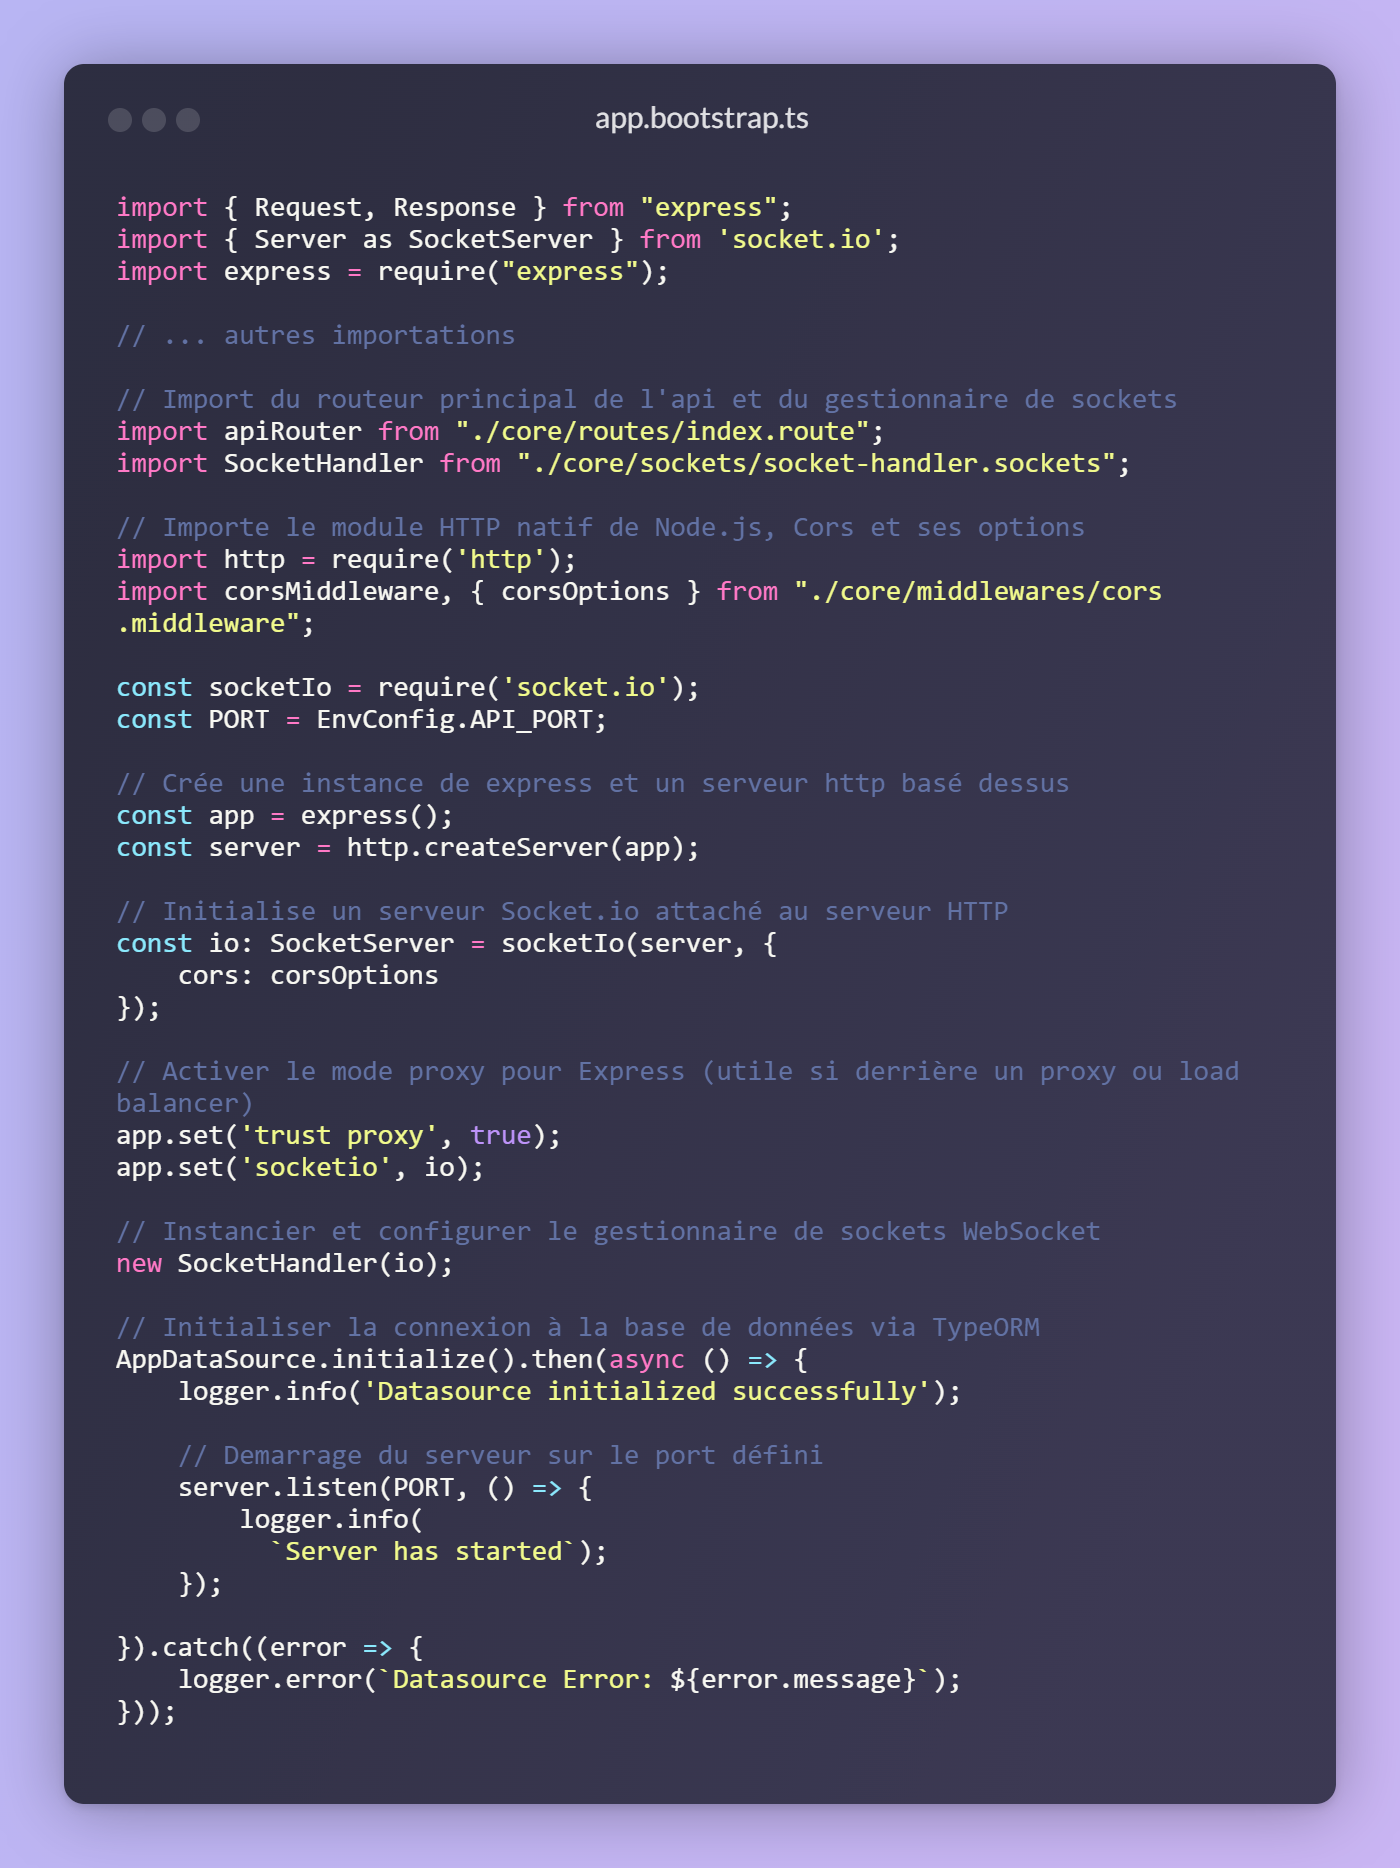
\includegraphics[width=15cm]{assets/annexes/snippet (13).png}
    \caption{ Exemple du point d'entrée de l'application}
\end{figure}

Ceci marque la dernière étape d'implémentation au backend. La prochaine étape consiste à implémenter la fonctionnalité côté frontend. 

\section{Module de Chat - Implémentation Côté Frontend}

L'implémentation côté frontend nécessite qu'on fasse dans un premier temps la structure HTML et CSS du chat. Pour les besoins de ce rapport, et afin d'éviter de faire un développement trop grand, nous allons survoler cette partie et mettre un accents sur les parties clées de l'implémentation frontend. La structure est de telle qu'elle est incluse dans un conteneur principal avec une classe \verb|main-content| et fond gris clair. Il contient une zone de chat principale qui se structure en deux colonnes flexibles :

\begin{enumerate}
    \item \textbf{La liste des conversations} (Panneau gauche) avec une liste déroulante des utilisateurs et un système d'onglets pour chaque conversation
    \item \textbf{Zone de conversation active} (Panneau droit) . Il se subdivise en plusieurs zone : 
    \begin{itemize}
        \item \textbf{En-tête de conversation} :contient l'avatar de l'utilisateur, le nom et le statut avec des boutons d'action (appel video, menu dropdown contenant des boutons profile et report, bouton de fermeture du chat)
        \item \textbf{Zone de message} : C'est un conteneur de liste non ordonnée de composants messages générés par javascript
        \item \textbf{Barre d'outil inférieurs} : Contient le bouton pour les pièces jointes, la zone de saisie de message, les boutons de fonctionnalité audio (enregistrement , timer, suppression d'enregistrement),
        bouton d'envoi de message
    \end{itemize}
\end{enumerate}

\vspace{0.35cm}

En plus de tout ce qui a été décrit, cette page définit aussi des composants modaux pour la gestion des appels (Modal d'appel entrant ou sortant, Modal d'appel en cours).

\vspace{0.35cm}

Notre structure au niveau des modules javascript inclu dans la page de chat se distingue en trois fichiers essentiels décrits ci-dessous : 

\begin{figure}[H]
    \centering
    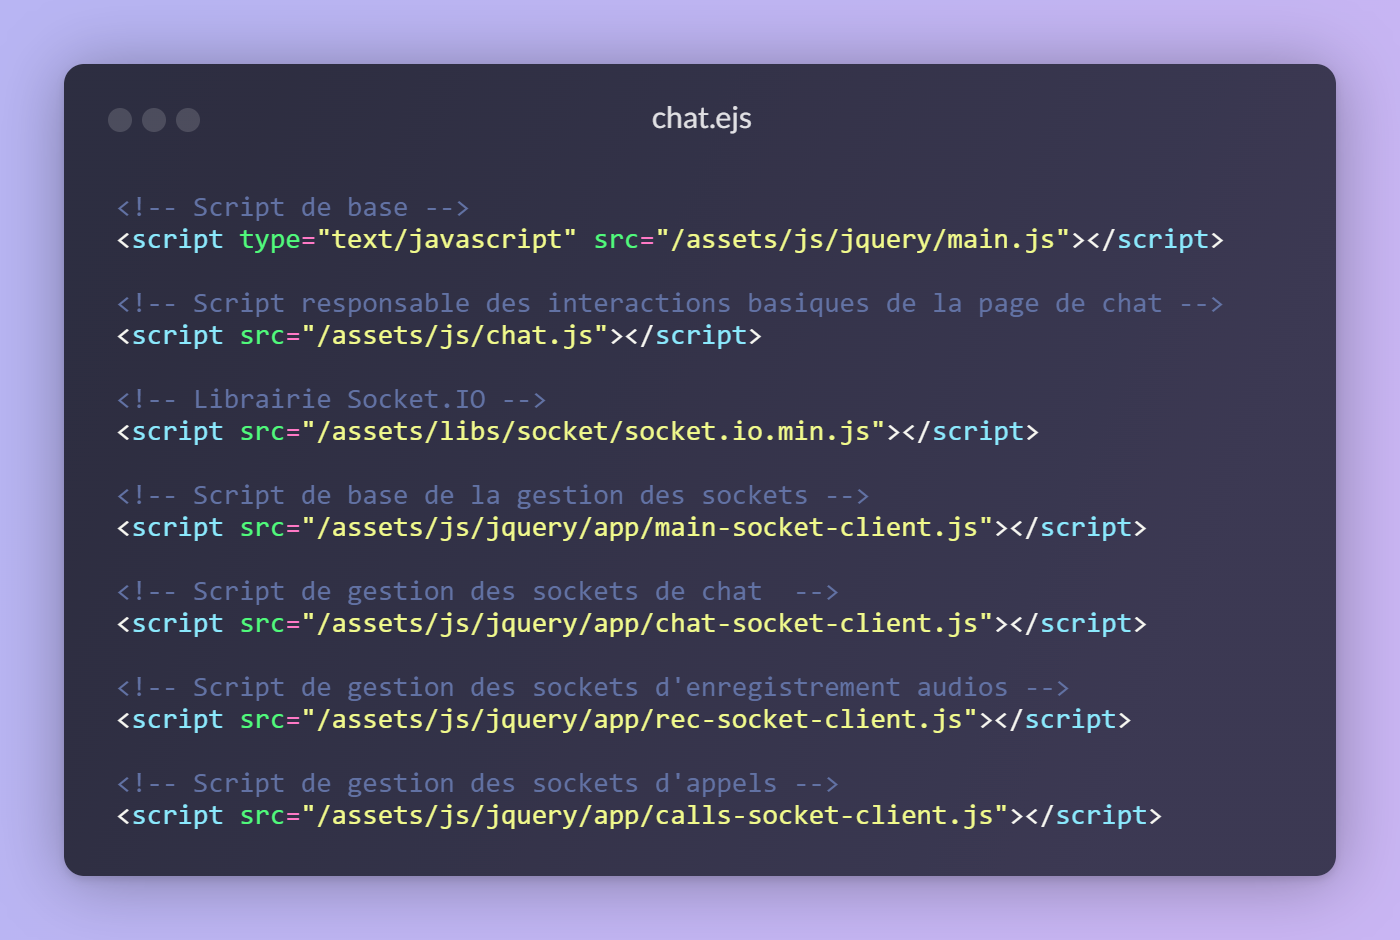
\includegraphics[width=15cm]{assets/annexes/snippet (14).png}
    \caption{ Scripts de gestion du chat}
\end{figure}

Les points clés dans l'implémentation de javascript de cette partie du projet sont les suivants : 

\vspace{0.35cm}

\subsection*{Gestion de la Connexion aux Sockets}

Dès le chargement de l'application, une connexion WebSocket est établie. L'utilisateur s'authentifie et rejoint automatiquement son salon de discussion.

\begin{figure}[H]
    \centering
    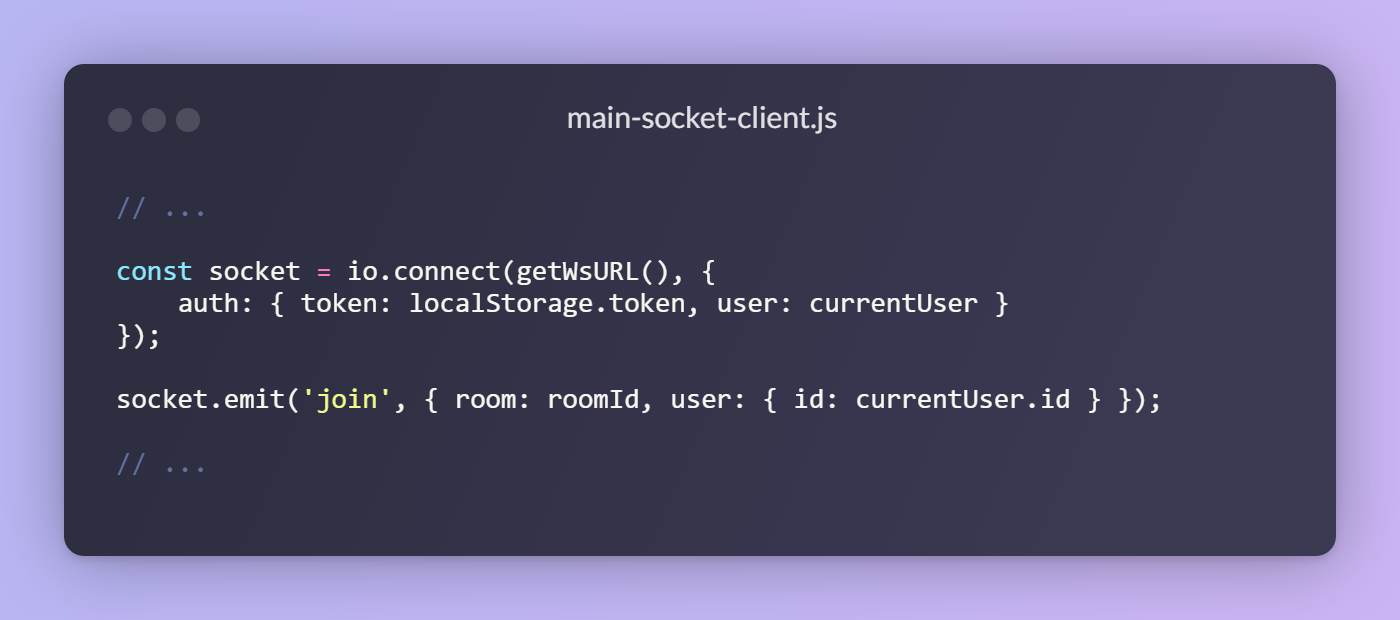
\includegraphics[width=15cm]{assets/annexes/snippet (15).png}
    \caption{ Gestion des connexions aux sockets}
\end{figure}

\subsection*{Envoi et Réception de Messages}

Les messages sont envoyés lorsqu’un utilisateur appuie sur Entrée ou clique sur le bouton d'envoi :

\begin{figure}[H]
    \centering
    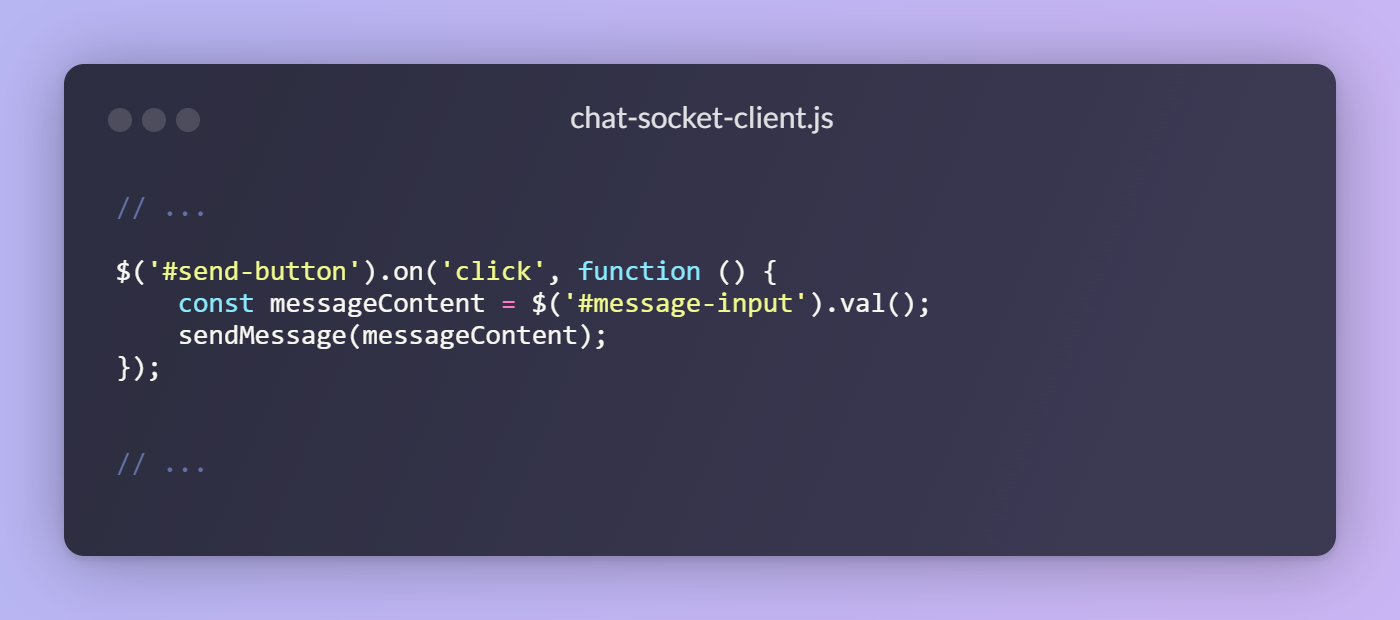
\includegraphics[width=15cm]{assets/annexes/snippet (16).png}
    \caption{ Envoi de message}
\end{figure}

À la réception d’un message, il est immédiatement affiché dans l’interface utilisateur :

\begin{figure}[H]
    \centering
    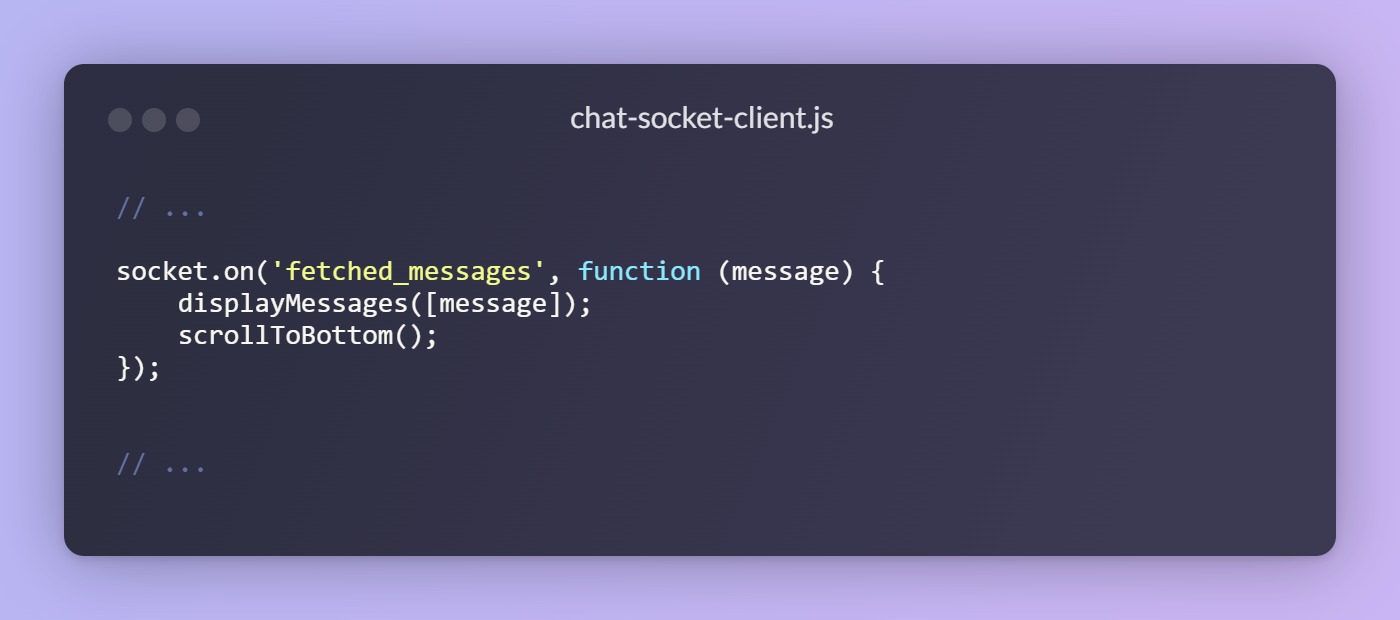
\includegraphics[width=15cm]{assets/annexes/snippet (17).png}
    \caption{ Affichage immédiat du message à la réception}
\end{figure}

\subsection*{Indicateur de Saisie (Typing Status)}

Lorsque l’utilisateur commence à écrire, un signal est envoyé aux autres participants du salon :

\begin{figure}[H]
    \centering
    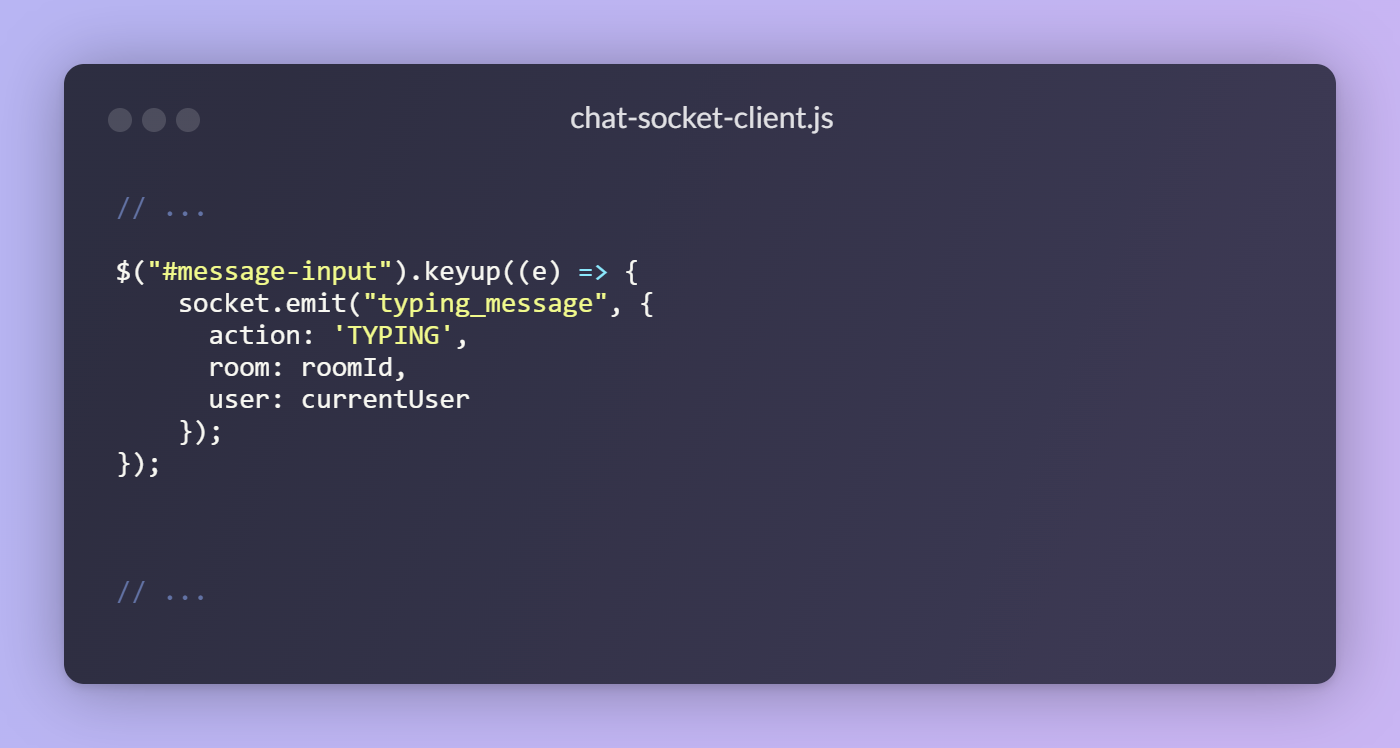
\includegraphics[width=15cm]{assets/annexes/snippet (18).png}
    \caption{ Signal de saisie en cours}
\end{figure}

L'affichage est mis à jour pour informer les autres utilisateurs :

\begin{figure}[H]
    \centering
    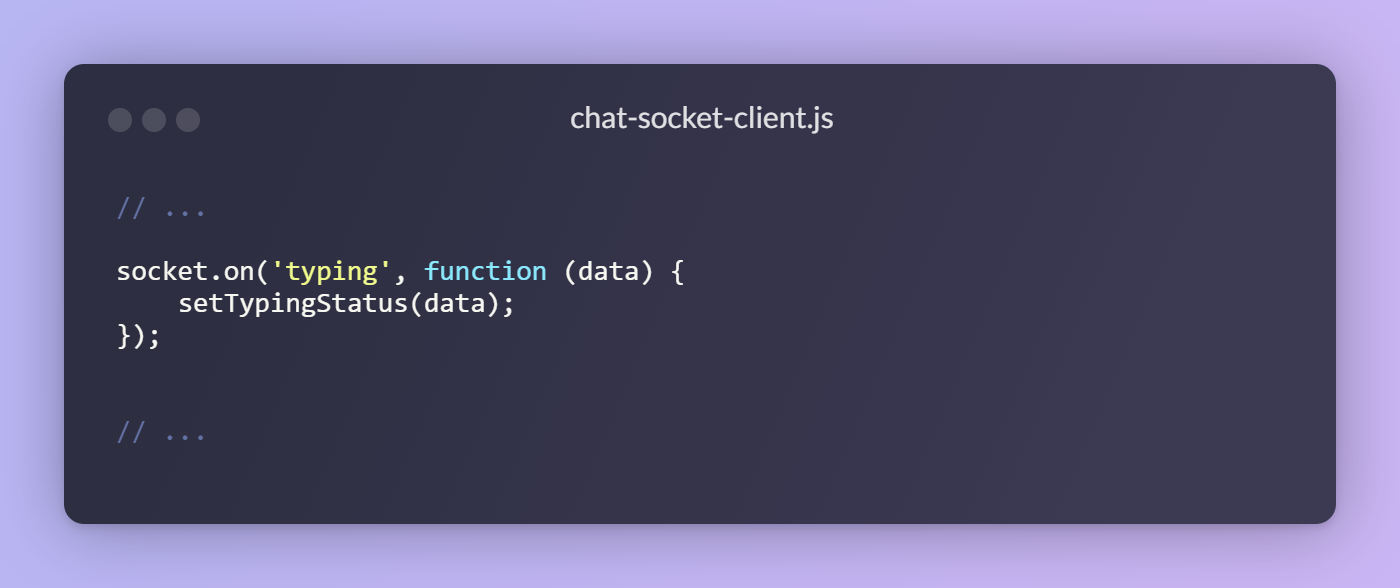
\includegraphics[width=15cm]{assets/annexes/snippet (19).png}
    \caption{ Mise à jour de l'indicateur de saisie}
\end{figure}

\subsection*{Envoi et Réception de Fichiers}

Les utilisateurs peuvent partager des fichiers en les convertissant en Base64 avant de les envoyer via WebSockets.

\begin{figure}[H]
    \centering
    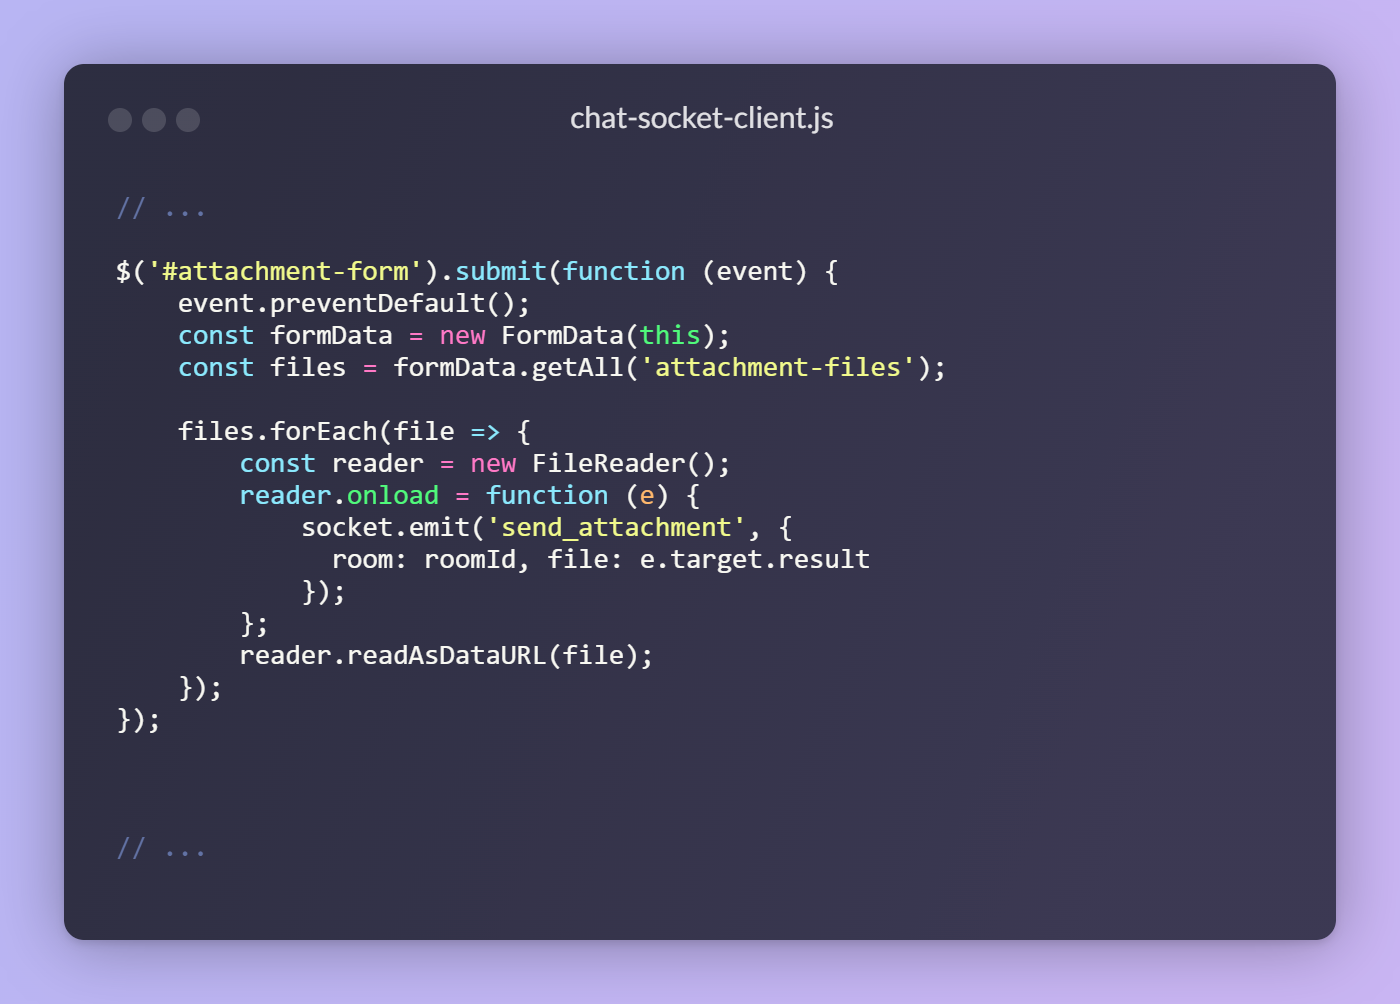
\includegraphics[width=15cm]{assets/annexes/snippet (20).png}
    \caption{ Envoi et Réception de Fichiers}
\end{figure}

\subsection*{Gestion des Appels Audio/Vidéo avec WebRTC - Initialisation de WebRTC}

Chaque utilisateur possède un peer ID unique généré avec PeerJS. Un serveur STUN est utilisé pour la traversée des NATs.

\begin{figure}[H]
    \centering
    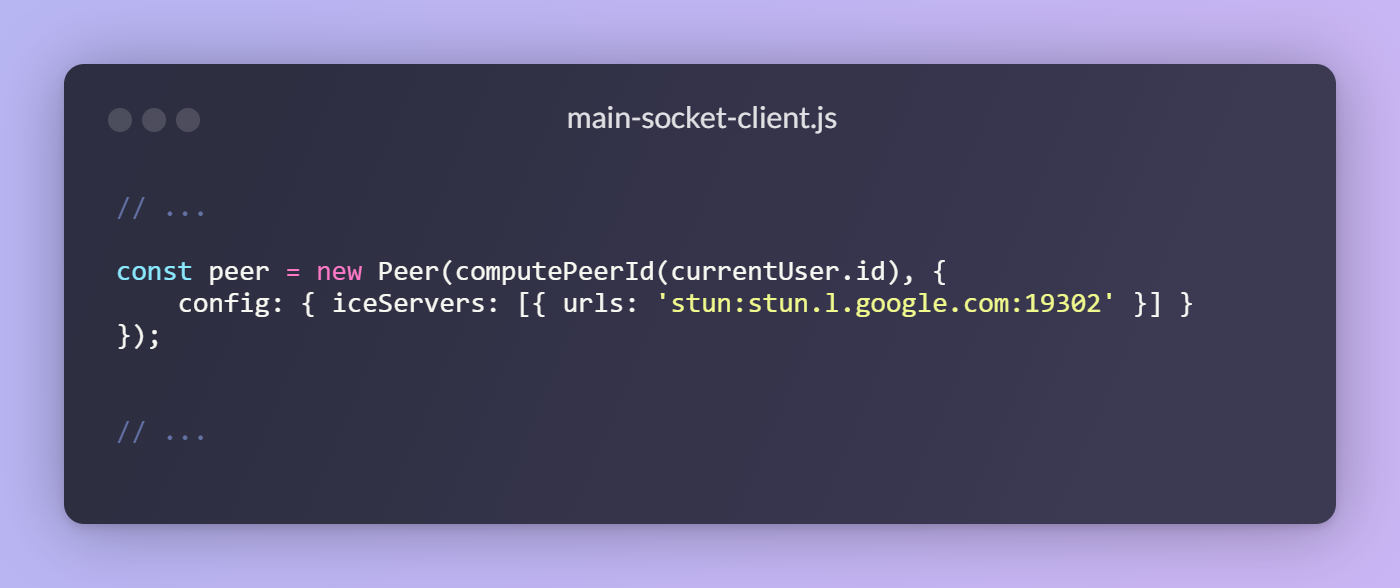
\includegraphics[width=15cm]{assets/annexes/snippet (21).png}
    \caption{ Initialisation du serveur STUN}
\end{figure}

Lorsqu'un utilisateur est prêt à recevoir des appels, il enregistre son peer ID sur le serveur :

\begin{figure}[H]
    \centering
    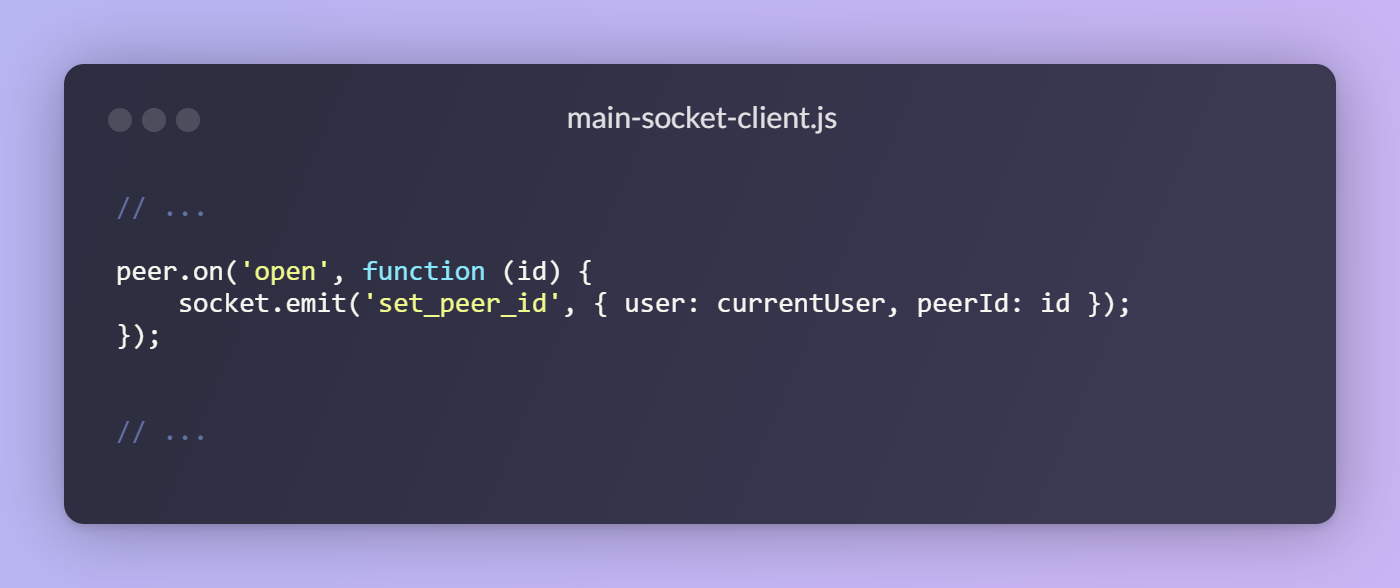
\includegraphics[width=15cm]{assets/annexes/snippet (22).png}
    \caption{ Enregistrement de Peer ID}
\end{figure}

\subsection*{Réception d’un Appel}

Lorsqu'un appel entrant est détecté, une sonnerie est jouée et une modalité d’appel s’affiche :

\begin{figure}[H]
    \centering
    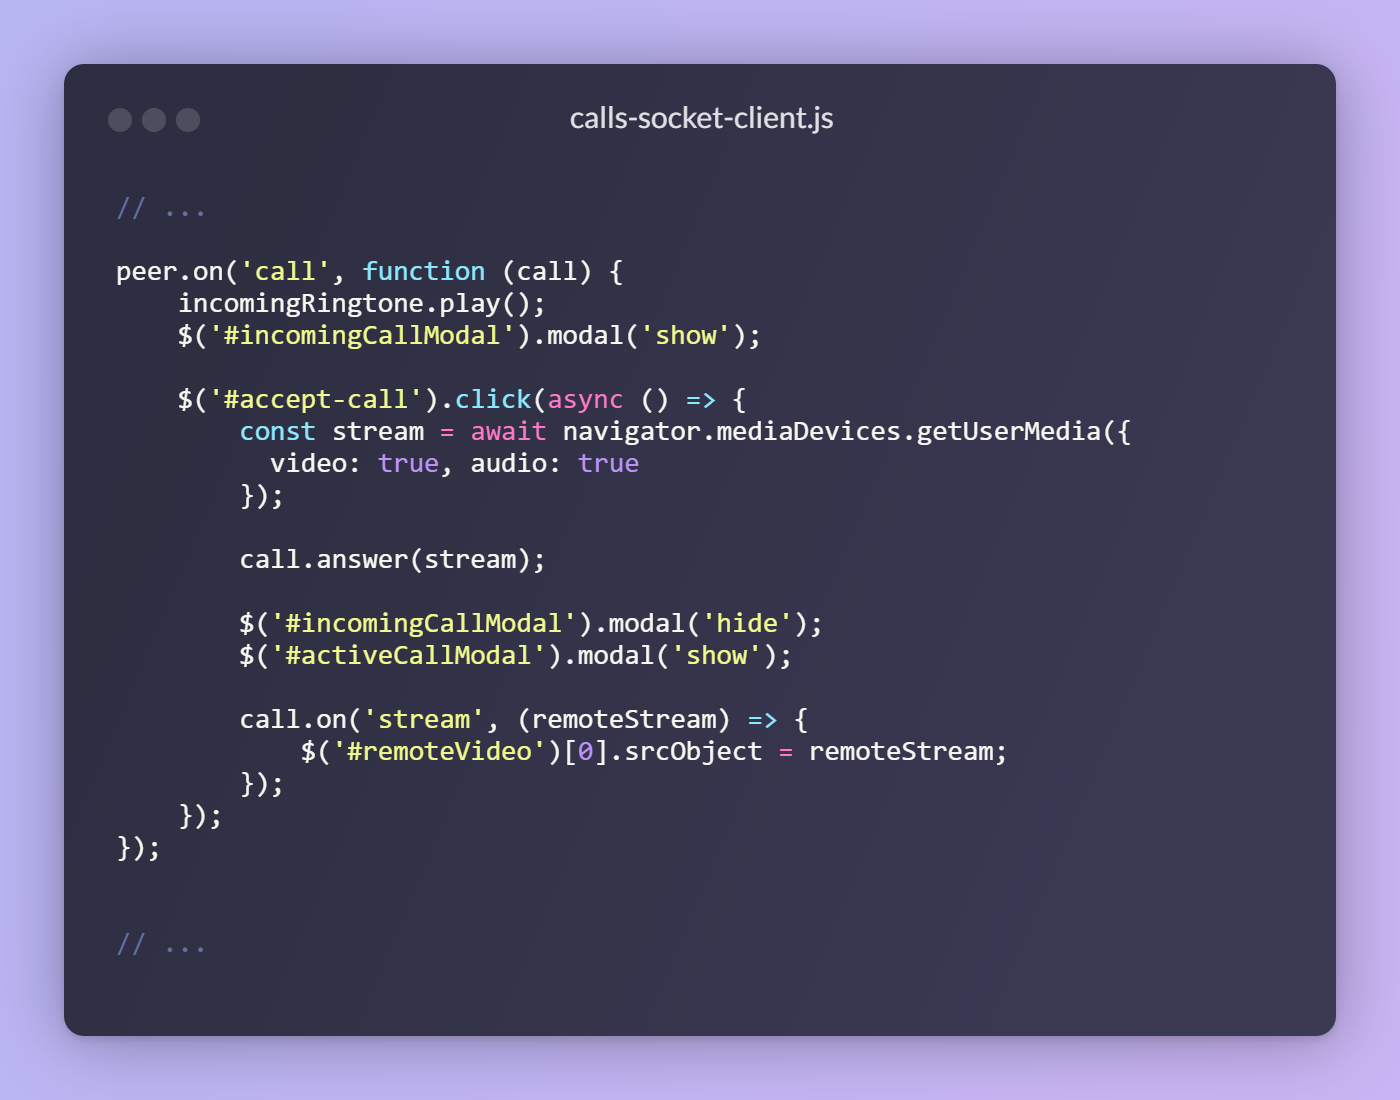
\includegraphics[width=15cm]{assets/annexes/snippet (23).png}
    \caption{ Réception d’un Appel}
\end{figure}

\subsection*{Passer un Appel}

L’utilisateur peut initier un appel audio ou vidéo en sélectionnant le type d’appel :

\begin{figure}[H]
    \centering
    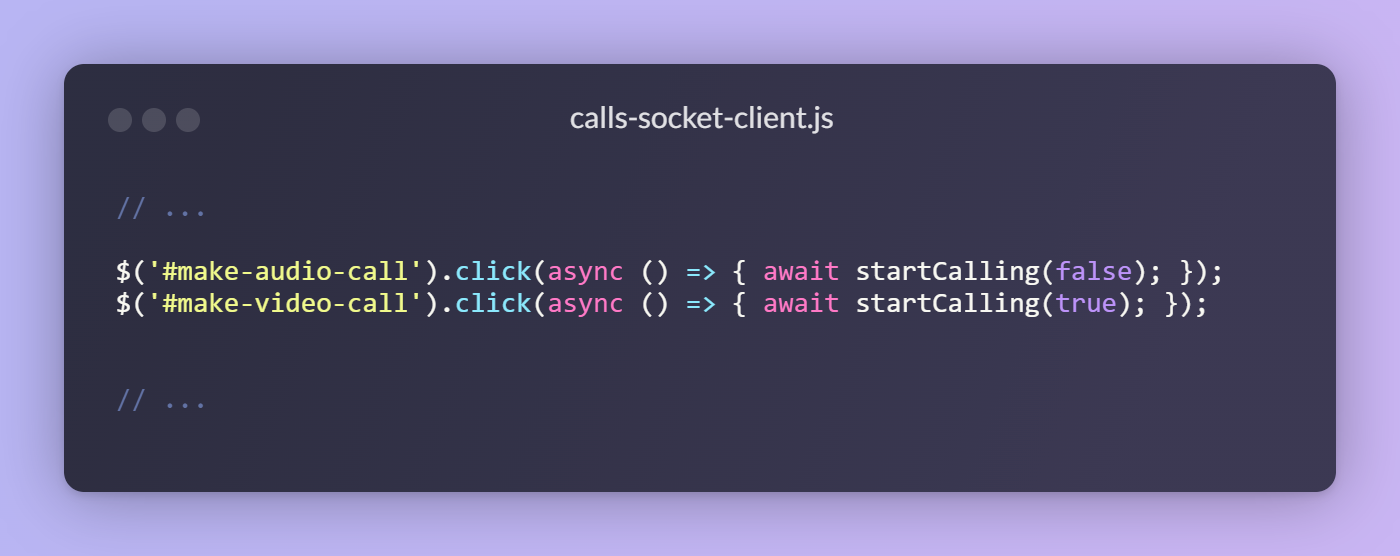
\includegraphics[width=15cm]{assets/annexes/snippet (24).png}
    \caption{ Initiation d'un appel}
\end{figure}

Une connexion WebRTC est alors établie avec l’interlocuteur :

\begin{figure}[H]
    \centering
    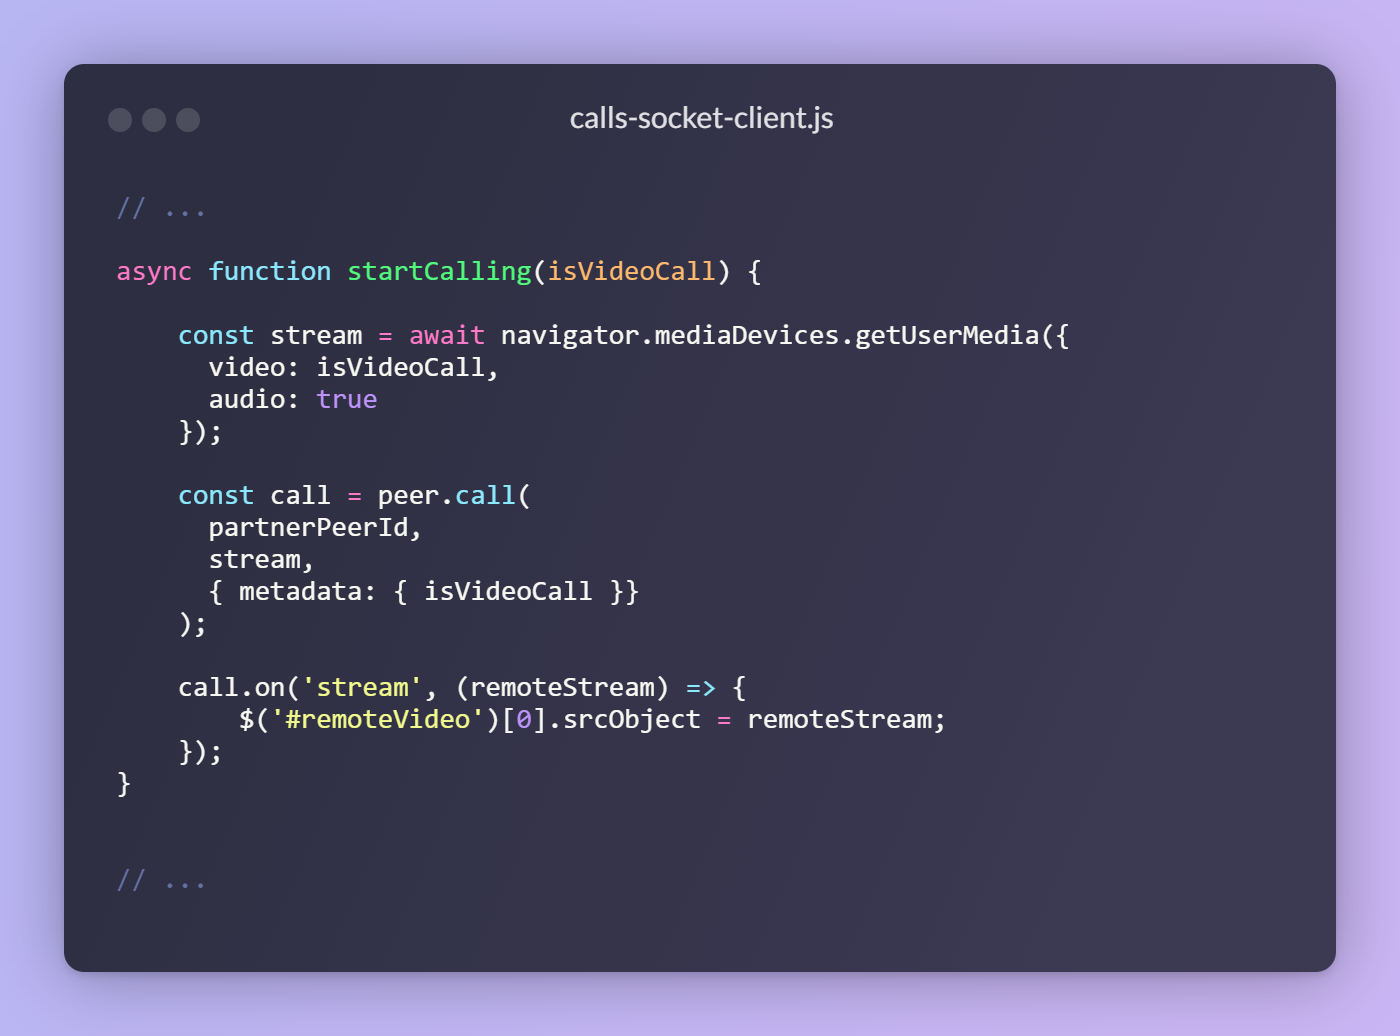
\includegraphics[width=15cm]{assets/annexes/snippet (25).png}
    \caption{ Etablissement de la connexion WebRTC}
\end{figure}


\subsection*{Terminer un Appel}

À la fin de l’appel, les flux médias sont arrêtés et les interfaces sont mises à jour :

\begin{figure}[H]
    \centering
    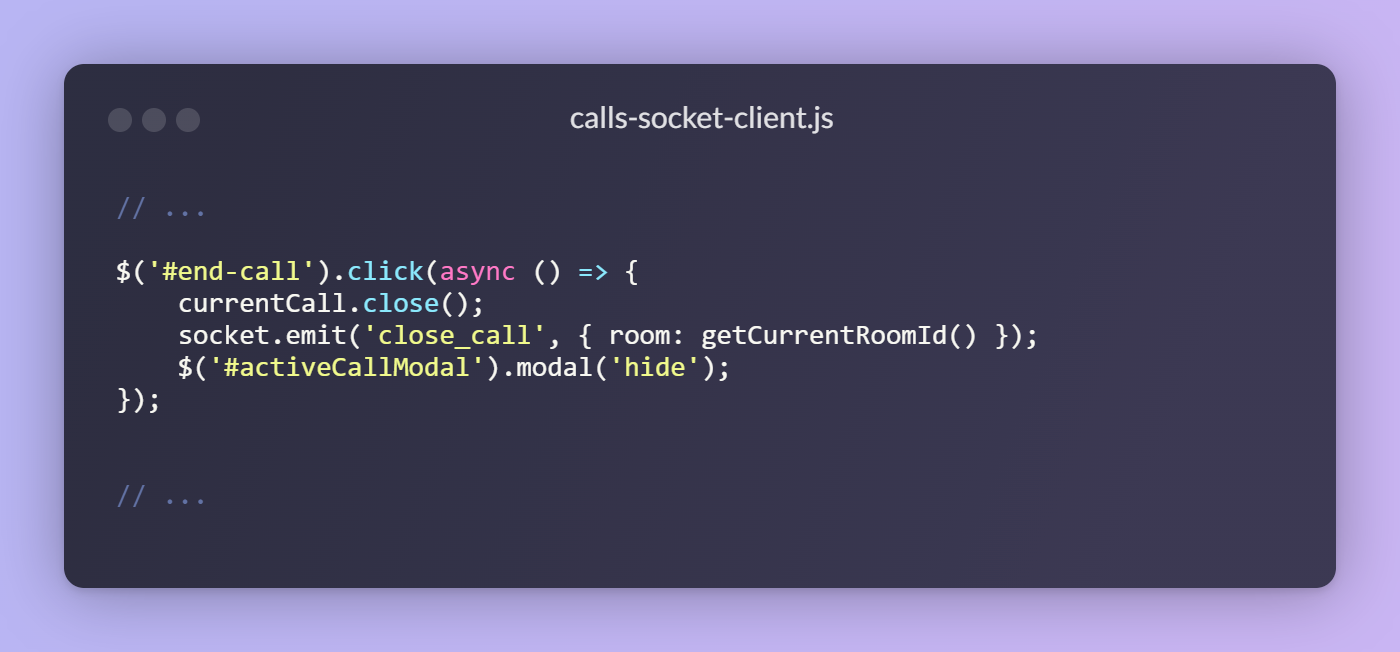
\includegraphics[width=15cm]{assets/annexes/snippet (26).png}
    \caption{ Terminer un appel}
\end{figure}

\subsection*{Affichage Dynamique des Messages et Notifications}

Les messages sont affichés en temps réel avec les informations de l’auteur :

\begin{figure}[H]
    \centering
    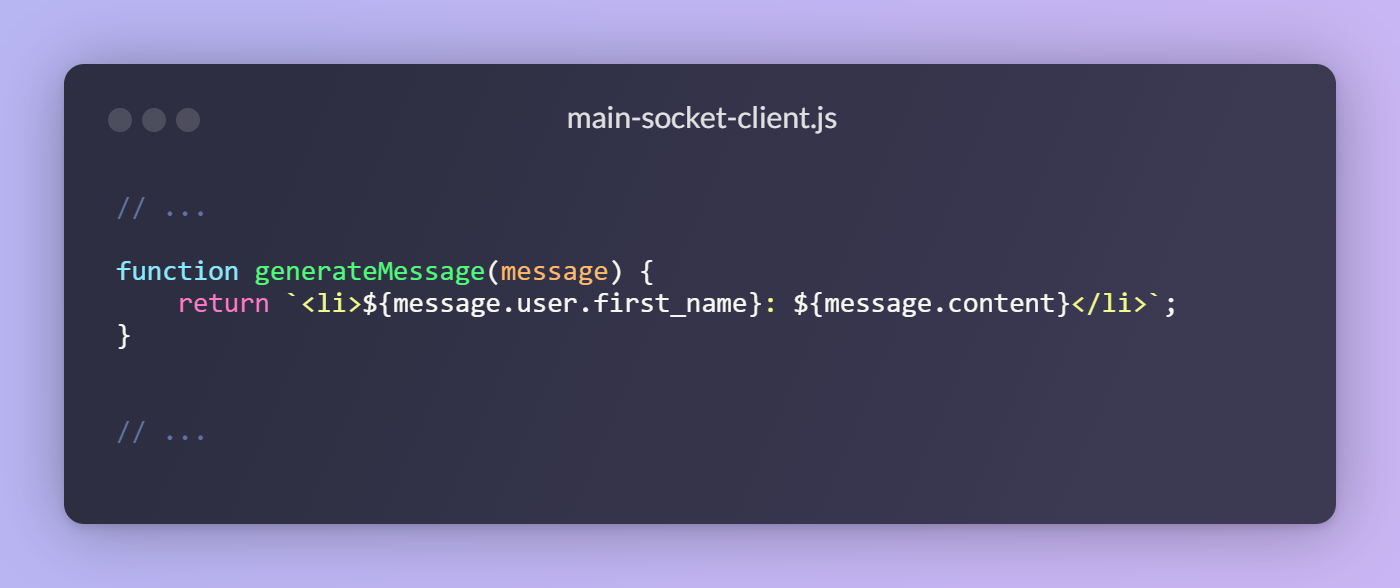
\includegraphics[width=15cm]{assets/annexes/snippet (27).png}
    \caption{ Methode de construction du message de notification}
\end{figure}

L’utilisateur reçoit également une notification lorsqu’un nouveau message arrive :

\begin{figure}[H]
    \centering
    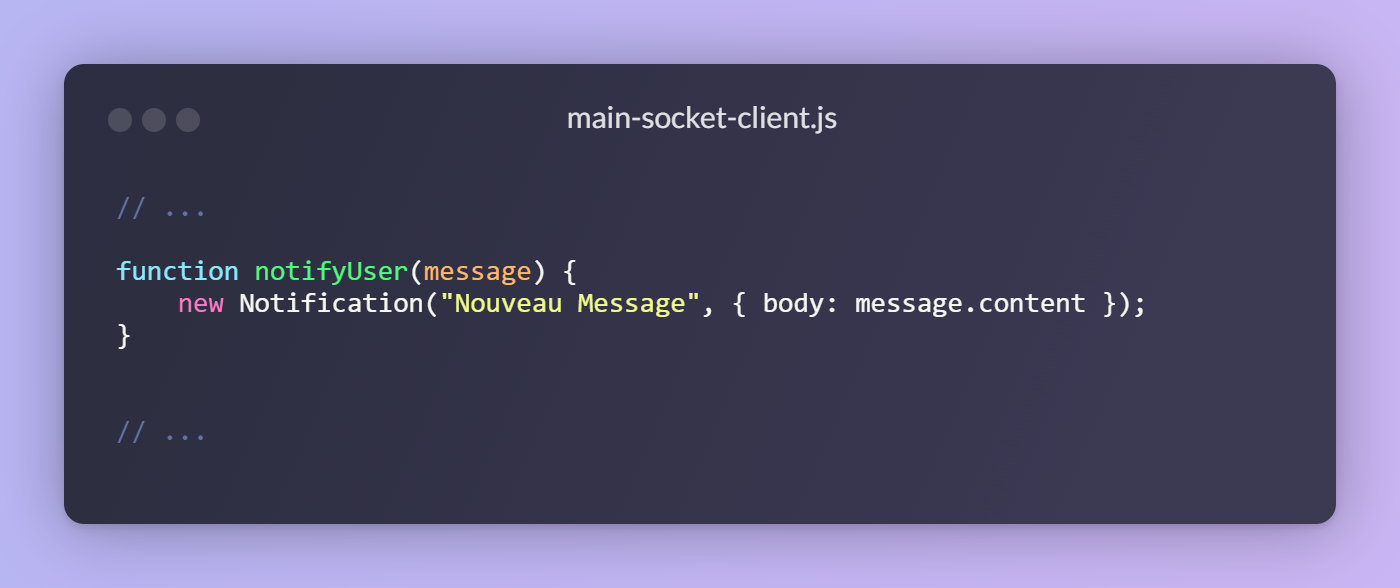
\includegraphics[width=15cm]{assets/annexes/snippet (28).png}
    \caption{ Réception de notification de message}
\end{figure}

\subsection*{Enregistrement et Envoi de Messages Audio}

Le système intègre une fonctionnalité d’enregistrement audio permettant aux utilisateurs d’envoyer des messages vocaux.

\vspace{0.35cm}

Lorsqu'un utilisateur clique sur le bouton d'enregistrement, l’application demande l'accès au microphone et démarre l’enregistrement via MediaRecorder.

\begin{figure}[H]
    \centering
    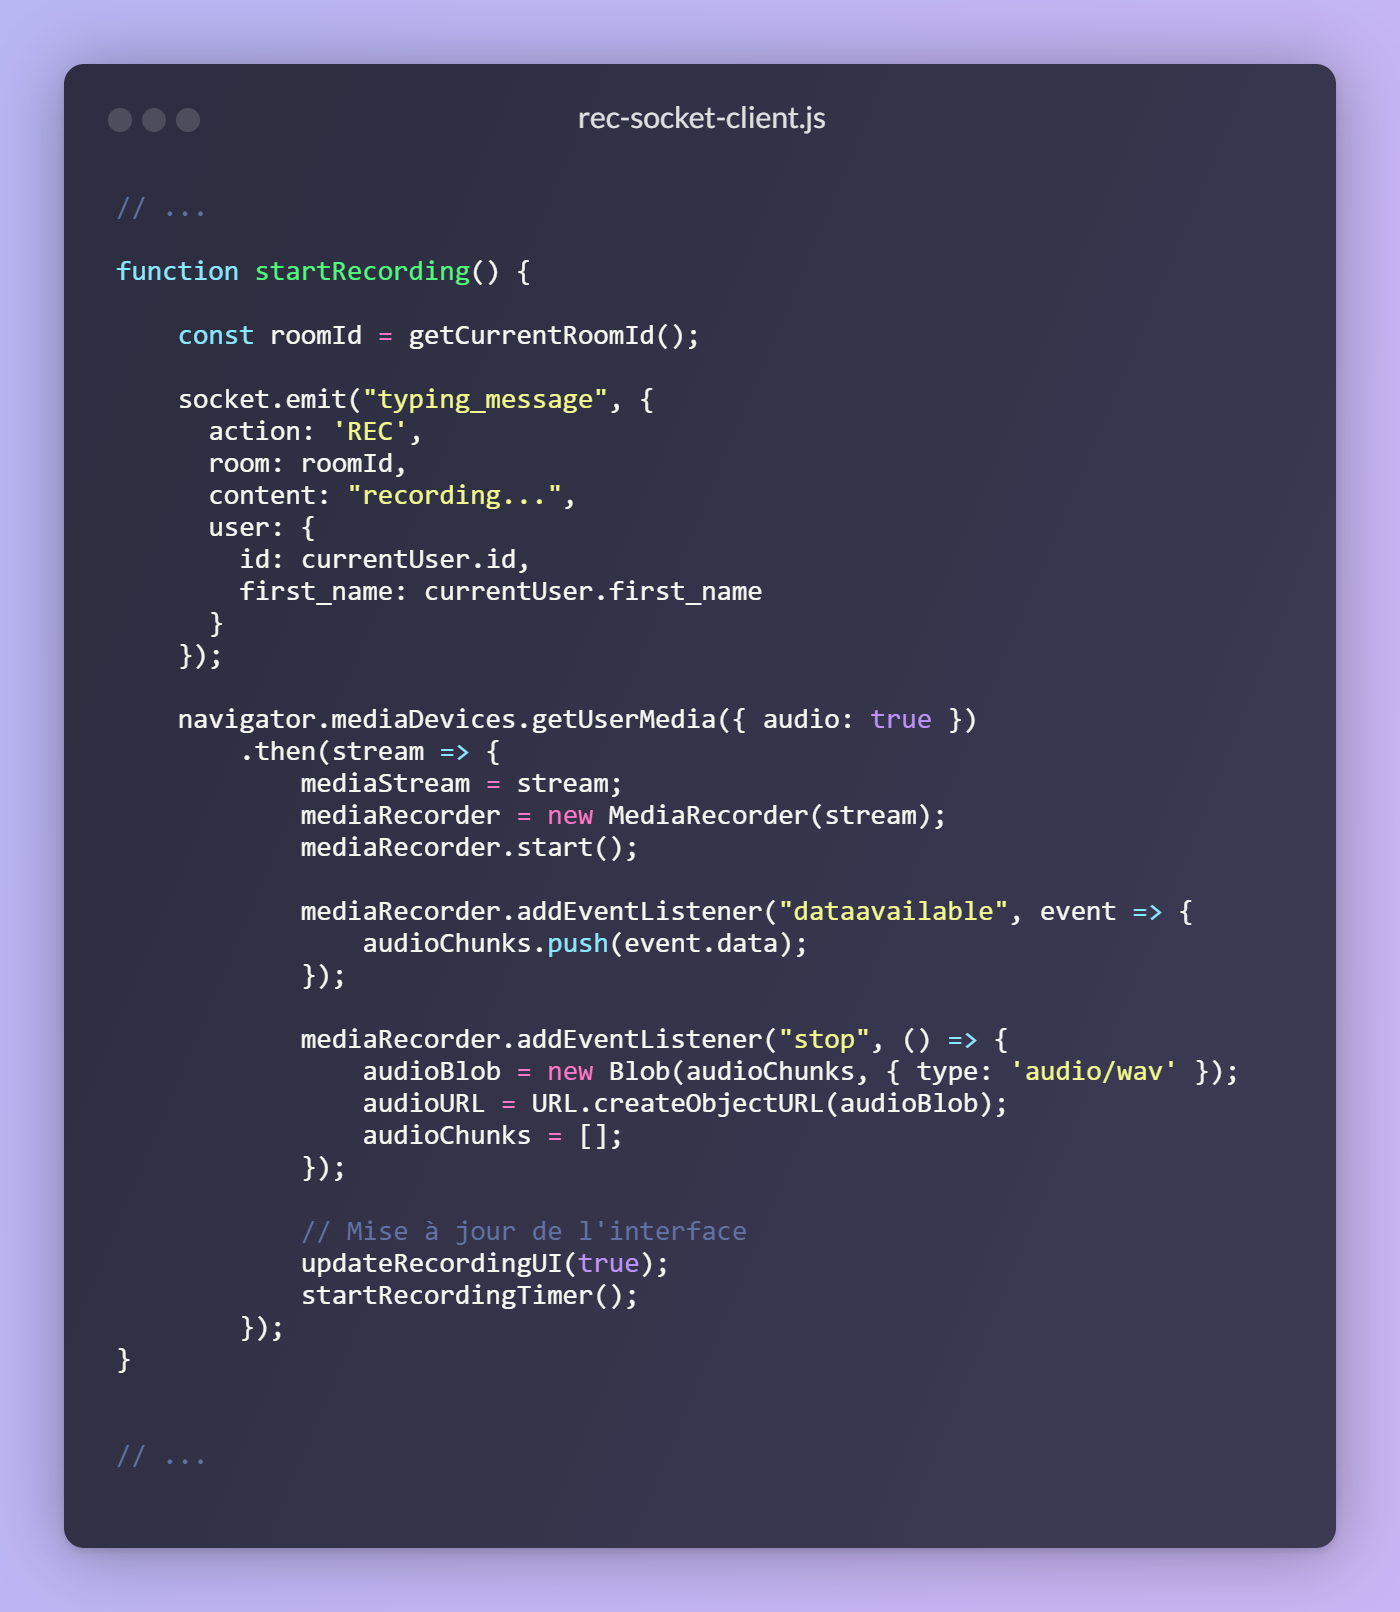
\includegraphics[width=15cm]{assets/annexes/snippet (29).png}
    \caption{ Démarrer l’Enregistrement}
\end{figure}

\begin{description}
    \item[Fonctionnalités implémentées par la méthode] :
    \begin{itemize}
        \item Envoi d’un signal de statut "Recording..." aux autres utilisateurs.
        \item Stockage des données audio sous forme de Blob.
        \item Masquage des éléments inutiles dans l'interface.
    \end{itemize}
\end{description}

\subsection*{Envoyer un Message Vocal}

Lorsque l'utilisateur termine l’enregistrement, le fichier est converti en Base64 et envoyé via Socket.io.

\begin{figure}[H]
    \centering
    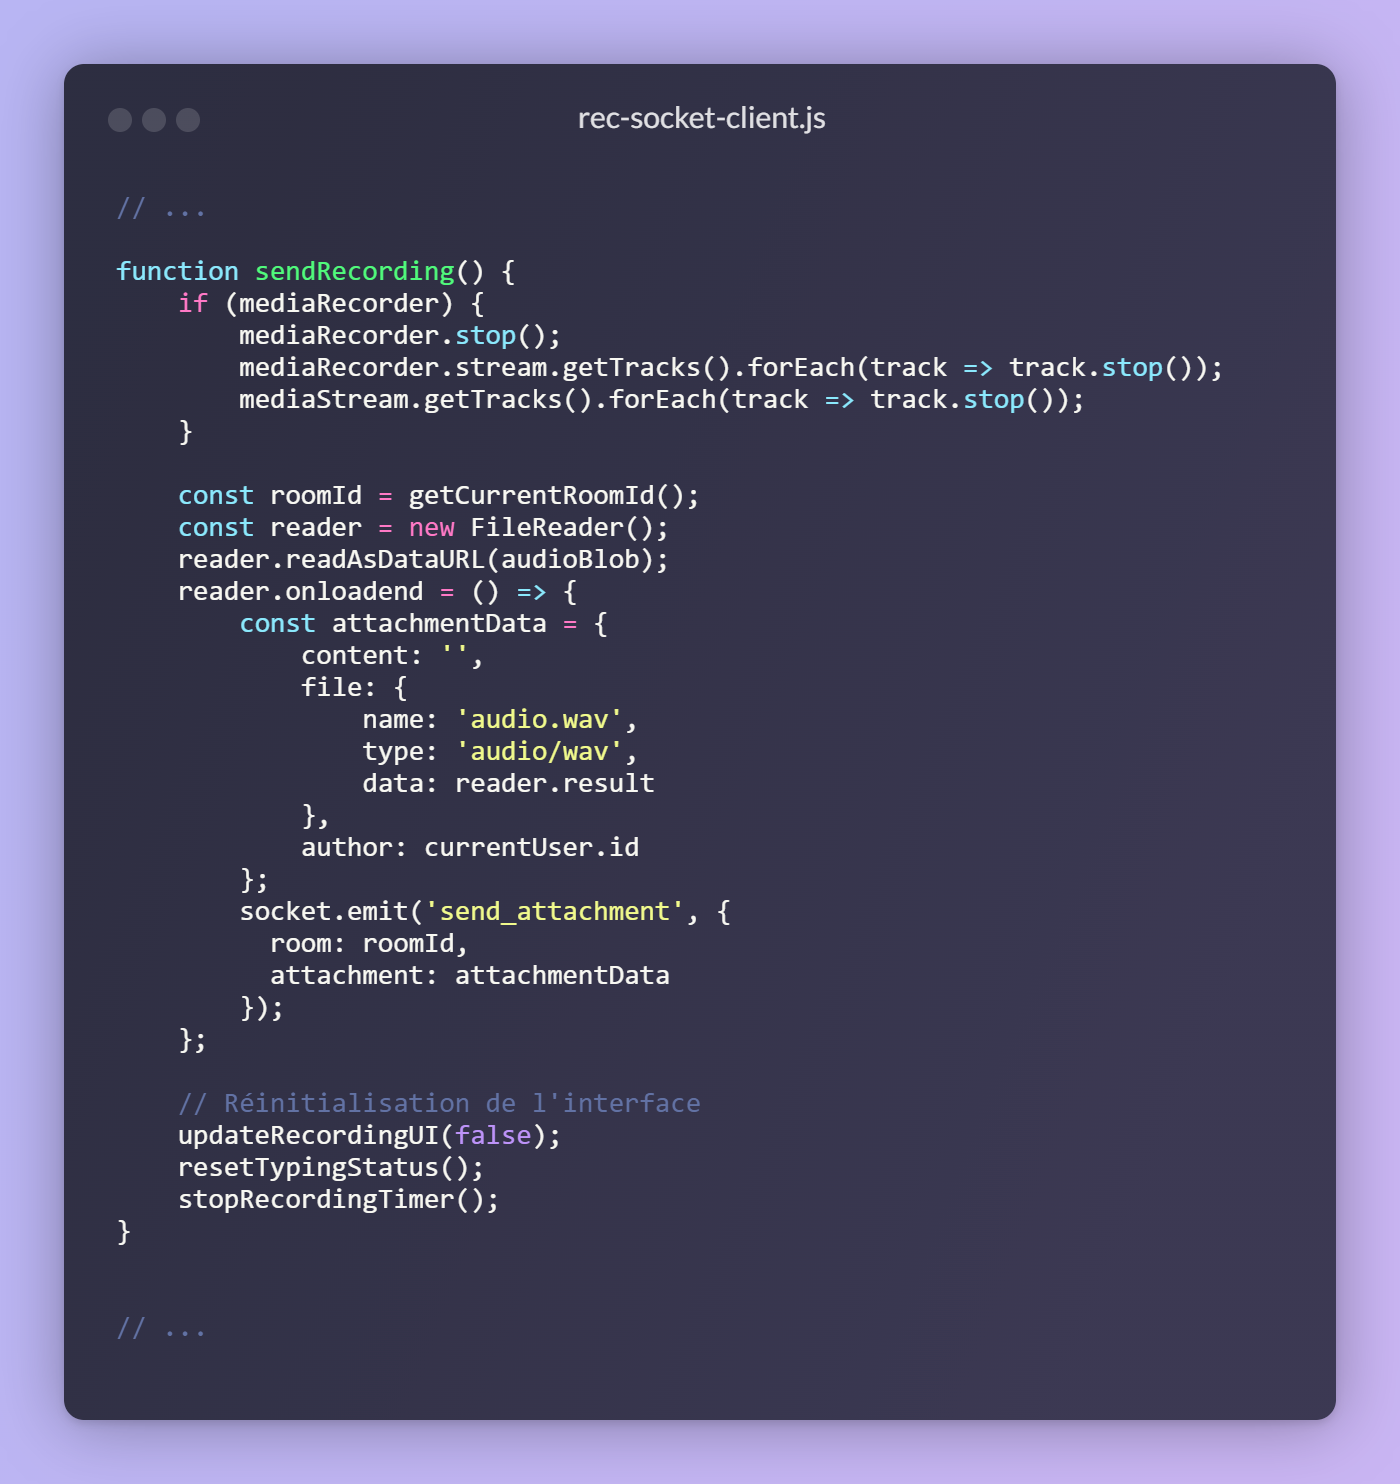
\includegraphics[width=15cm]{assets/annexes/snippet (30).png}
    \caption{ Envoyer un Message Vocal}
\end{figure}

\begin{description}
    \item[Détails importants] :
    \begin{itemize}
        \item L’enregistrement est arrêté et converti en fichier Base64
        \item Le fichier est envoyé au serveur WebSocket
        \item L’interface est réinitialisée.
    \end{itemize}
\end{description}


\subsection*{Supprimer un Enregistrement}

L'utilisateur peut annuler un enregistrement avant l'envoi :

\begin{figure}[H]
    \centering
    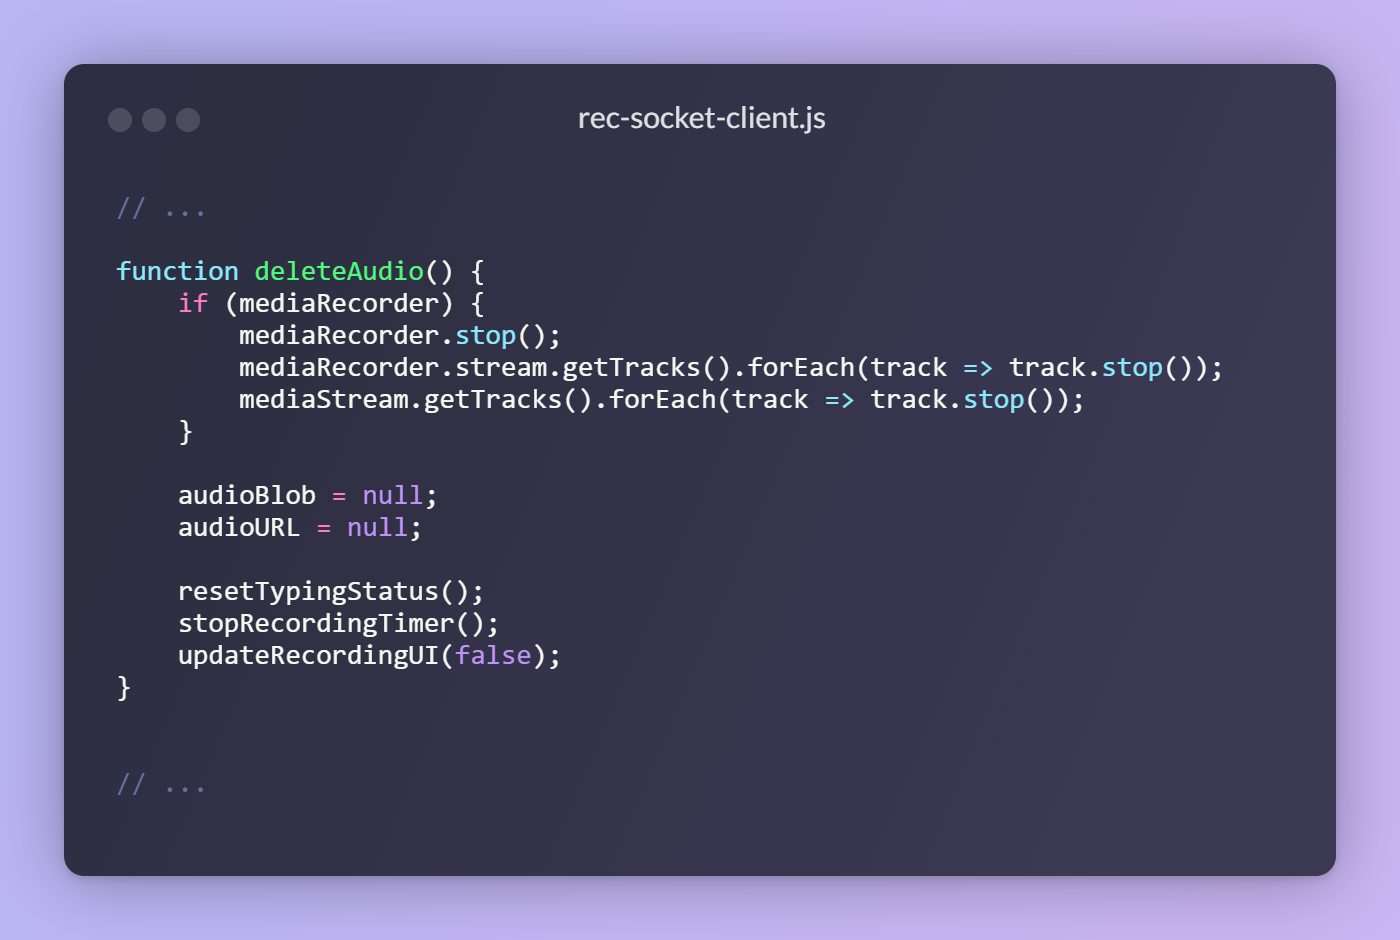
\includegraphics[width=15cm]{assets/annexes/snippet (31).png}
    \caption{ Supprimer un Enregistrement}
\end{figure}

\subsection*{Gestion du Timer d’Enregistrement}

Un compteur de temps s'affiche pour indiquer la durée de l'enregistrement :

\begin{figure}[H]
    \centering
    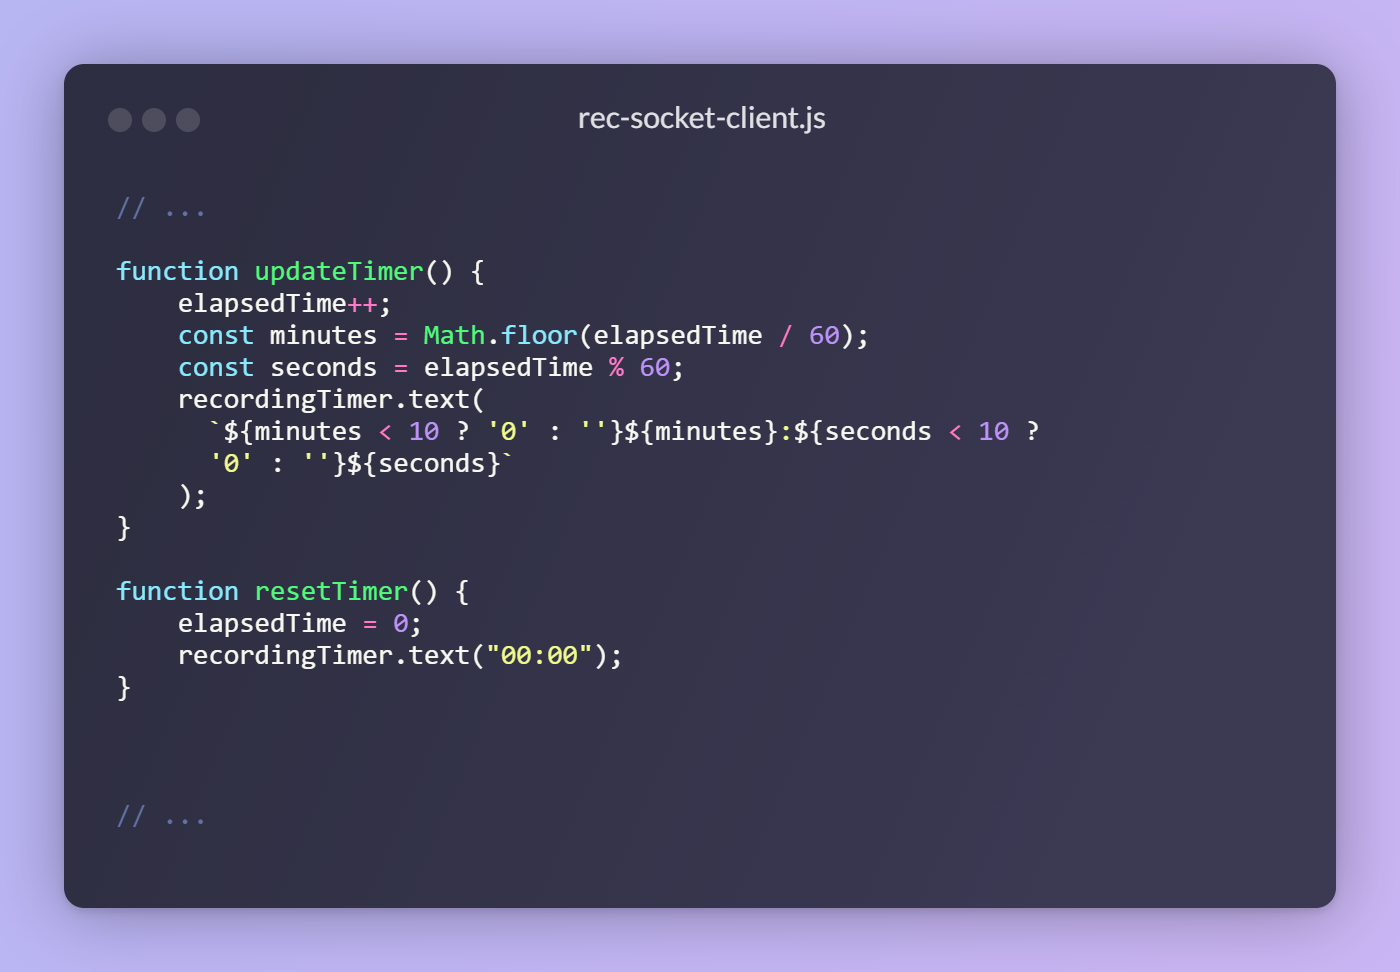
\includegraphics[width=15cm]{assets/annexes/snippet (32).png}
    \caption{ Gestion du Timer d’Enregistrement}
\end{figure}


\subsection*{Mise à Jour Dynamique de l’Interface}

Lors de l'enregistrement ou de l'envoi, certains boutons sont cachés ou affichés :

\begin{figure}[H]
    \centering
    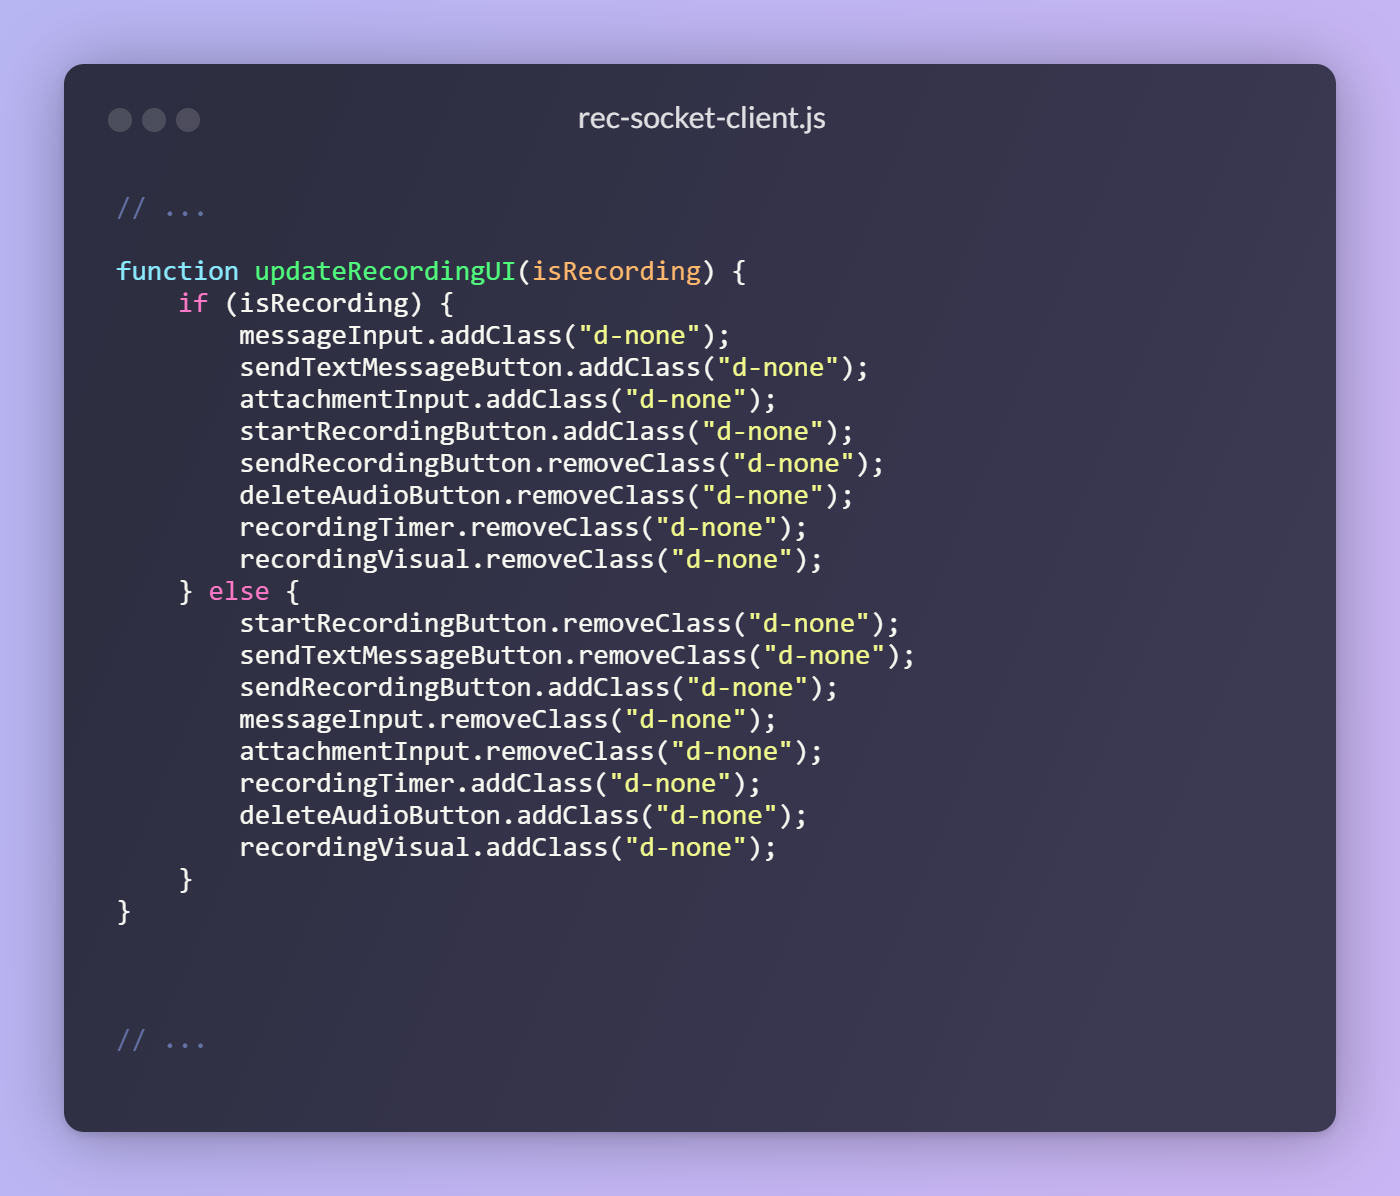
\includegraphics[width=15cm]{assets/annexes/snippet (33).png}
    \caption{ Mise à Jour Dynamique de l’Interface}
\end{figure}
